\documentclass[twoside]{book}

% Packages required by doxygen
\usepackage{fixltx2e}
\usepackage{calc}
\usepackage{doxygen}
\usepackage[export]{adjustbox} % also loads graphicx
\usepackage{graphicx}
\usepackage[utf8]{inputenc}
\usepackage{makeidx}
\usepackage{multicol}
\usepackage{multirow}
\PassOptionsToPackage{warn}{textcomp}
\usepackage{textcomp}
\usepackage[nointegrals]{wasysym}
\usepackage[table]{xcolor}

% Font selection
\usepackage[T1]{fontenc}
\usepackage[scaled=.90]{helvet}
\usepackage{courier}
\usepackage{amssymb}
\usepackage{sectsty}
\renewcommand{\familydefault}{\sfdefault}
\allsectionsfont{%
  \fontseries{bc}\selectfont%
  \color{darkgray}%
}
\renewcommand{\DoxyLabelFont}{%
  \fontseries{bc}\selectfont%
  \color{darkgray}%
}
\newcommand{\+}{\discretionary{\mbox{\scriptsize$\hookleftarrow$}}{}{}}

% Page & text layout
\usepackage{geometry}
\geometry{%
  a4paper,%
  top=2.5cm,%
  bottom=2.5cm,%
  left=2.5cm,%
  right=2.5cm%
}
\tolerance=750
\hfuzz=15pt
\hbadness=750
\setlength{\emergencystretch}{15pt}
\setlength{\parindent}{0cm}
\setlength{\parskip}{3ex plus 2ex minus 2ex}
\makeatletter
\renewcommand{\paragraph}{%
  \@startsection{paragraph}{4}{0ex}{-1.0ex}{1.0ex}{%
    \normalfont\normalsize\bfseries\SS@parafont%
  }%
}
\renewcommand{\subparagraph}{%
  \@startsection{subparagraph}{5}{0ex}{-1.0ex}{1.0ex}{%
    \normalfont\normalsize\bfseries\SS@subparafont%
  }%
}
\makeatother

% Headers & footers
\usepackage{fancyhdr}
\pagestyle{fancyplain}
\fancyhead[LE]{\fancyplain{}{\bfseries\thepage}}
\fancyhead[CE]{\fancyplain{}{}}
\fancyhead[RE]{\fancyplain{}{\bfseries\leftmark}}
\fancyhead[LO]{\fancyplain{}{\bfseries\rightmark}}
\fancyhead[CO]{\fancyplain{}{}}
\fancyhead[RO]{\fancyplain{}{\bfseries\thepage}}
\fancyfoot[LE]{\fancyplain{}{}}
\fancyfoot[CE]{\fancyplain{}{}}
\fancyfoot[RE]{\fancyplain{}{\bfseries\scriptsize Generated by Doxygen }}
\fancyfoot[LO]{\fancyplain{}{\bfseries\scriptsize Generated by Doxygen }}
\fancyfoot[CO]{\fancyplain{}{}}
\fancyfoot[RO]{\fancyplain{}{}}
\renewcommand{\footrulewidth}{0.4pt}
\renewcommand{\chaptermark}[1]{%
  \markboth{#1}{}%
}
\renewcommand{\sectionmark}[1]{%
  \markright{\thesection\ #1}%
}

% Indices & bibliography
\usepackage{natbib}
\usepackage[titles]{tocloft}
\setcounter{tocdepth}{3}
\setcounter{secnumdepth}{5}
\makeindex

% Hyperlinks (required, but should be loaded last)
\usepackage{ifpdf}
\ifpdf
  \usepackage[pdftex,pagebackref=true]{hyperref}
\else
  \usepackage[ps2pdf,pagebackref=true]{hyperref}
\fi
\hypersetup{%
  colorlinks=true,%
  linkcolor=blue,%
  citecolor=blue,%
  unicode%
}

% Custom commands
\newcommand{\clearemptydoublepage}{%
  \newpage{\pagestyle{empty}\cleardoublepage}%
}

\usepackage{caption}
\captionsetup{labelsep=space,justification=centering,font={bf},singlelinecheck=off,skip=4pt,position=top}

%===== C O N T E N T S =====

\begin{document}

% Titlepage & ToC
\hypersetup{pageanchor=false,
             bookmarksnumbered=true,
             pdfencoding=unicode
            }
\pagenumbering{alph}
\begin{titlepage}
\vspace*{7cm}
\begin{center}%
{\Large M\+A\+GL Micromouse }\\
\vspace*{1cm}
{\large Generated by Doxygen 1.8.13}\\
\end{center}
\end{titlepage}
\clearemptydoublepage
\pagenumbering{roman}
\tableofcontents
\clearemptydoublepage
\pagenumbering{arabic}
\hypersetup{pageanchor=true}

%--- Begin generated contents ---
\chapter{Micromouse}
\label{md_README}
\Hypertarget{md_README}
This software was deveoped by Nicholas Appleton and Christian Woof of U\+WE Robotics. It is for use with a micromouse with a ds\+P\+I\+C30\+F4011 microcontroller, with the pin-\/layout as shown in Fig. 1. It is desined with compliance to the micromouse international competition. The maze that it was created to solve is an 8x6 maze, however, the size of the maze can be set accordingly and the actual size of the maze does not need to be known, as long as the size is set to greater than the actual size. A simulator is also included in the code so that the functionality can be tested without a physical mouse. To use the simulator, the integration folder should be excluded from the project, and the S\+I\+M\+U\+L\+A\+T\+OR macro set to 1. A series of test mazes can be found later in this document, these should be pasted into the \hyperlink{simulator_8c}{simulator.\+c} file.



The \hyperlink{structMaze}{Maze} contains a high level algorithm that maps the maze by pushing any cell it finds to an openlist of unexplored cells, from which the most recently found is explored. A nodemap is created where Nodes are created and destroyed as necissary to the final solving. Various functionality is shown in Fig. 2.



Fig. 3 shows the interaction between the high level algorithm and the low level integration code.



\section*{Test Mazes}

Test mazes for use in the simulated environment. Each maze focusses on tripping up the algorithm in a different way.

1) \{0,1,1,1, 0,1,1,1, 0,1,1,1, 0,1,1,1, 0,1,1,1, 0,1,1,1\}, \{0,0,0,1, 0,1,0,0, 0,1,0,1, 0,1,0,1, 0,1,0,1, 0,1,0,1\}, \{0,1,0,1, 0,0,0,1, 1,0,0,0, 0,0,0,0, 1,0,0,0, 0,1,0,0\}, \{0,1,0,1, 1,1,0,1, 0,0,1,1, 0,1,0,0, 0,1,1,1, 0,1,0,1\}, \{0,1,0,1, 0,1,1,1, 1,0,0,1, 1,1,0,0, 0,0,0,1, 0,1,0,0\}, \{0,1,0,1, 1,0,0,1, 1,0,1,0, 1,0,1,0, 1,1,0,0, 0,1,0,1\}, \{0,0,0,1, 1,0,1,0, 1,0,1,0, 0,0,1,0, 1,0,1,0, 0,1,0,0\}, \{1,0,0,1, 1,0,1,0, 1,1,1,0, 1,1,0,1, 1,0,1,1, 1,1,0,0\}

2) \{0,1,1,1, 0,0,1,1, 0,0,1,0, 0,0,1,0, 0,1,1,0, 0,1,1,1\}, \{0,0,0,1, 0,1,0,0, 0,1,0,1, 0,1,0,1, 0,1,0,1, 0,1,0,1\}, \{0,1,0,1, 0,0,0,1, 1,0,0,1, 1,0,0,0, 0,1,0,0, 0,1,0,1\}, \{0,0,0,1, 0,1,0,0, 0,0,1,1, 0,1,1,0, 0,1,0,1, 0,1,0,1\}, \{0,1,0,1, 0,1,0,1, 1,0,0,1, 1,0,0,0, 0,1,0,0, 0,1,0,1\}, \{0,0,0,1, 0,0,0,0, 1,0,1,0, 0,0,1,0, 1,0,0,0, 0,1,0,0\}, \{0,1,0,1, 1,0,0,1, 0,1,1,0, 0,0,0,1, 0,0,1,0, 0,1,0,0\}, \{1,0,1,1, 1,0,1,0, 1,0,0,0, 1,1,0,0, 1,1,0,1, 1,1,0,1\}

3) \{0,1,1,1, 0,0,1,1, 0,1,1,0, 0,0,1,1, 1,0,1,0, 0,1,1,0\}, \{0,1,0,1, 0,1,0,1, 0,1,0,1, 0,1,0,1, 0,0,1,1, 1,1,0,0\}, \{0,1,0,1, 0,1,0,1, 1,0,0,1, 1,1,0,0, 1,0,0,1, 0,1,1,0\}, \{0,1,0,1, 0,1,0,1, 0,0,1,1, 0,0,1,0, 0,1,1,0, 0,1,0,1\}, \{0,1,0,1, 0,1,0,1, 1,0,0,1, 1,1,0,0, 0,1,0,1, 0,1,0,1\}, \{0,1,0,1, 0,1,0,1, 0,0,1,1, 0,1,1,0, 0,1,0,1, 0,1,0,1\}, \{0,1,0,1, 1,0,0,1, 1,1,0,0, 1,0,0,1, 1,1,0,0, 0,1,0,1\}, \{1,0,0,1, 1,0,1,0, 1,0,1,0, 1,0,1,0, 1,0,1,0, 1,1,0,0\}

4) \{0,1,1,1, 0,0,1,1, 0,0,1,0, 1,0,1,0, 0,1,1,0, 0,1,1,1\}, \{1,0,0,1, 0,1,0,0, 0,1,0,1, 0,0,1,1, 1,1,0,0, 0,1,0,1\}, \{0,0,1,1, 1,0,1,0, 1,0,0,0, 1,0,0,0, 0,0,1,0, 1,1,0,0\}, \{0,1,0,1, 0,0,1,1, 0,0,1,0, 0,1,1,0, 0,1,0,1, 0,1,1,1\}, \{0,0,0,1, 1,1,0,0, 1,0,0,1, 1,1,0,0, 0,1,0,1, 0,1,0,1\}, \{1,0,0,1, 0,1,1,0, 0,0,1,1, 0,0,1,0, 0,0,0,0, 0,1,0,0\}, \{0,1,1,1, 1,0,0,1, 1,1,0,0, 0,1,0,1, 0,1,0,1, 0,1,0,1\}, \{1,0,0,1, 1,0,1,0, 1,0,1,0, 1,1,0,0, 1,1,0,1, 1,1,0,1\}

5) \{0,1,1,1, 0,1,1,1, 0,1,1,1, 0,0,1,1, 1,0,1,0, 0,1,1,0\}, \{0,0,0,1, 0,0,0,0, 0,0,0,0, 0,0,0,0, 1,0,1,0, 0,1,0,0\}, \{0,1,0,1, 0,1,0,1, 1,1,0,1, 1,0,0,1, 0,1,1,0, 0,1,0,1\}, \{0,1,0,1, 0,1,0,1, 0,0,1,1, 0,1,1,0, 0,1,0,1, 0,1,0,1\}, \{0,1,0,1, 0,1,0,1, 0,0,0,1, 1,1,0,0, 0,1,0,1, 0,1,0,1\}, \{0,1,0,1, 1,0,0,1, 0,1,0,0, 0,0,1,1, 1,0,0,0, 0,1,0,0\}, \{0,0,0,1, 1,1,1,0, 1,0,0,1, 0,0,0,0, 1,0,1,0, 0,1,0,0\}, \{1,1,0,1, 1,0,1,1, 1,0,1,0, 1,0,0,0, 1,0,1,0, 1,1,0,0\}

6) \{0,1,1,1, 0,0,1,1, 1,1,1,0, 0,0,1,1, 1,1,1,0, 0,1,1,1\}, \{0,0,0,1, 0,0,0,0, 1,0,1,0, 0,1,0,0, 0,1,1,1, 0,1,0,1\}, \{0,1,0,1, 0,0,0,1, 1,1,1,0, 1,0,0,1, 0,0,0,0, 0,1,0,0\}, \{1,1,0,1, 0,1,0,1, 0,0,1,1, 0,1,1,0, 0,1,0,1, 0,1,0,1\}, \{0,0,1,1, 1,1,0,0, 0,0,0,1, 1,1,0,0, 1,1,0,1, 0,1,0,1\}, \{0,1,0,1, 0,1,1,1, 0,1,0,1, 0,0,1,1, 1,0,1,0, 0,1,0,0\}, \{1,0,0,1, 0,0,0,0, 0,0,0,0, 1,0,0,0, 1,0,1,0, 0,1,0,0\}, \{1,0,1,1, 1,1,0,1, 1,0,0,1, 1,0,1,0, 1,0,1,0, 1,1,0,0\} 
\chapter{Class Index}
\section{Class List}
Here are the classes, structs, unions and interfaces with brief descriptions\+:\begin{DoxyCompactList}
\item\contentsline{section}{\hyperlink{structcell}{cell} \\*All info about a given cell }{\pageref{structcell}}{}
\item\contentsline{section}{\hyperlink{structconnection}{connection} \\*Connection between 2 nodes }{\pageref{structconnection}}{}
\item\contentsline{section}{\hyperlink{structMaze}{Maze} \\*Contains the representation of the maze itself }{\pageref{structMaze}}{}
\item\contentsline{section}{\hyperlink{structMouse}{Mouse} \\*Representation of the \hyperlink{structMouse}{Mouse} in virtual space }{\pageref{structMouse}}{}
\item\contentsline{section}{\hyperlink{structNode}{Node} \\*All info about a given \hyperlink{structNode}{Node} }{\pageref{structNode}}{}
\item\contentsline{section}{\hyperlink{structStack}{Stack} \\*Array of data that is the \hyperlink{structStack}{Stack} }{\pageref{structStack}}{}
\end{DoxyCompactList}

\chapter{File Index}
\section{File List}
Here is a list of all documented files with brief descriptions\+:\begin{DoxyCompactList}
\item\contentsline{section}{\hyperlink{main_8c}{main.\+c} \\*This is the main file that controls the robot }{\pageref{main_8c}}{}
\item\contentsline{section}{\hyperlink{Stacks_8h}{Stacks.\+h} \\*Defines everything needed to implement stacks }{\pageref{Stacks_8h}}{}
\item\contentsline{section}{Algorithm/\hyperlink{Dijekstra_8h}{Dijekstra.\+h} \\*Dijekstra\textquotesingle{}s function and cocktail sort }{\pageref{Dijekstra_8h}}{}
\item\contentsline{section}{Algorithm/\hyperlink{MapMaze_8c}{Map\+Maze.\+c} \\*Fully maps the maze }{\pageref{MapMaze_8c}}{}
\item\contentsline{section}{Algorithm/{\bfseries Map\+Maze.\+h} }{\pageref{MapMaze_8h}}{}
\item\contentsline{section}{Algorithm/\hyperlink{MappingFunctions_8h}{Mapping\+Functions.\+h} \\*All functions, structures and data types used by most files }{\pageref{MappingFunctions_8h}}{}
\item\contentsline{section}{Algorithm/\hyperlink{simulator_8c}{simulator.\+c} \\*Display the maze for debugging }{\pageref{simulator_8c}}{}
\item\contentsline{section}{Algorithm/{\bfseries simulator.\+h} }{\pageref{simulator_8h}}{}
\item\contentsline{section}{Integration/\hyperlink{IO_8c}{I\+O.\+c} \\*Functions for input and output Integration }{\pageref{IO_8c}}{}
\item\contentsline{section}{Integration/{\bfseries I\+O.\+h} }{\pageref{IO_8h}}{}
\item\contentsline{section}{Integration/\hyperlink{Motors_8c}{Motors.\+c} \\*Motor Functions and Defines }{\pageref{Motors_8c}}{}
\item\contentsline{section}{Integration/{\bfseries Motors.\+h} }{\pageref{Motors_8h}}{}
\item\contentsline{section}{Integration/\hyperlink{Setup_8c}{Setup.\+c} \\*Functions and Definitions for peripheral systems }{\pageref{Setup_8c}}{}
\item\contentsline{section}{Integration/{\bfseries Setup.\+h} }{\pageref{Setup_8h}}{}
\end{DoxyCompactList}

\chapter{Class Documentation}
\hypertarget{structcell}{}\section{cell Struct Reference}
\label{structcell}\index{cell@{cell}}


All info about a given cell.  




{\ttfamily \#include $<$Mapping\+Functions.\+h$>$}



Collaboration diagram for cell\+:
\nopagebreak
\begin{figure}[H]
\begin{center}
\leavevmode
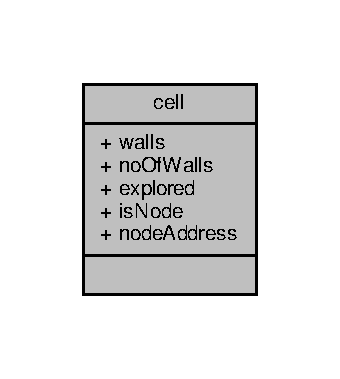
\includegraphics[width=163pt]{structcell__coll__graph}
\end{center}
\end{figure}
\subsection*{Public Attributes}
\begin{DoxyCompactItemize}
\item 
unsigned int \hyperlink{structcell_a9a2929dcb308b9eb30f19cddebcc5c52}{walls}\+: 4
\item 
unsigned int \hyperlink{structcell_a8d23cc3f76831a9bcf536b77ba272848}{no\+Of\+Walls}\+: 6
\item 
unsigned int \hyperlink{structcell_aefc3f7506ad8c2ad9f31e7d9ba093828}{explored}\+: 1
\item 
unsigned int \hyperlink{structcell_aaa0cb97f34f5d696c6d7f2ef154fbfc8}{is\+Node}\+: 1
\item 
unsigned char \hyperlink{structcell_a0b372a9239a2ed20cde6edb427069bd8}{node\+Address}
\end{DoxyCompactItemize}


\subsection{Detailed Description}
All info about a given cell. 

\subsection{Member Data Documentation}
\mbox{\Hypertarget{structcell_aefc3f7506ad8c2ad9f31e7d9ba093828}\label{structcell_aefc3f7506ad8c2ad9f31e7d9ba093828}} 
\index{cell@{cell}!explored@{explored}}
\index{explored@{explored}!cell@{cell}}
\subsubsection{\texorpdfstring{explored}{explored}}
{\footnotesize\ttfamily unsigned int cell\+::explored}

Marks whether cell has been visited \mbox{\Hypertarget{structcell_aaa0cb97f34f5d696c6d7f2ef154fbfc8}\label{structcell_aaa0cb97f34f5d696c6d7f2ef154fbfc8}} 
\index{cell@{cell}!is\+Node@{is\+Node}}
\index{is\+Node@{is\+Node}!cell@{cell}}
\subsubsection{\texorpdfstring{is\+Node}{isNode}}
{\footnotesize\ttfamily unsigned int cell\+::is\+Node}

Marks whether cell is a \hyperlink{structNode}{Node} or not \mbox{\Hypertarget{structcell_a0b372a9239a2ed20cde6edb427069bd8}\label{structcell_a0b372a9239a2ed20cde6edb427069bd8}} 
\index{cell@{cell}!node\+Address@{node\+Address}}
\index{node\+Address@{node\+Address}!cell@{cell}}
\subsubsection{\texorpdfstring{node\+Address}{nodeAddress}}
{\footnotesize\ttfamily unsigned char cell\+::node\+Address}

Index of \hyperlink{structNode}{Node} that references this cell in nodelist \mbox{\Hypertarget{structcell_a8d23cc3f76831a9bcf536b77ba272848}\label{structcell_a8d23cc3f76831a9bcf536b77ba272848}} 
\index{cell@{cell}!no\+Of\+Walls@{no\+Of\+Walls}}
\index{no\+Of\+Walls@{no\+Of\+Walls}!cell@{cell}}
\subsubsection{\texorpdfstring{no\+Of\+Walls}{noOfWalls}}
{\footnotesize\ttfamily unsigned int cell\+::no\+Of\+Walls}

Number of walls of cell. can never be more than 4 \mbox{\Hypertarget{structcell_a9a2929dcb308b9eb30f19cddebcc5c52}\label{structcell_a9a2929dcb308b9eb30f19cddebcc5c52}} 
\index{cell@{cell}!walls@{walls}}
\index{walls@{walls}!cell@{cell}}
\subsubsection{\texorpdfstring{walls}{walls}}
{\footnotesize\ttfamily unsigned int cell\+::walls}

Layout of walls; 1 denotes a wall, 0 is no wall. bit-\/order is N$>$E$>$S$>$W 

The documentation for this struct was generated from the following file\+:\begin{DoxyCompactItemize}
\item 
Algorithm/\hyperlink{MappingFunctions_8h}{Mapping\+Functions.\+h}\end{DoxyCompactItemize}

\hypertarget{structconnection}{}\section{connection Struct Reference}
\label{structconnection}\index{connection@{connection}}


Connection between 2 nodes.  




{\ttfamily \#include $<$Mapping\+Functions.\+h$>$}



Collaboration diagram for connection\+:
\nopagebreak
\begin{figure}[H]
\begin{center}
\leavevmode
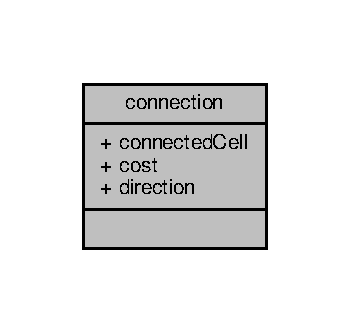
\includegraphics[width=168pt]{structconnection__coll__graph}
\end{center}
\end{figure}
\subsection*{Public Attributes}
\begin{DoxyCompactItemize}
\item 
unsigned char \hyperlink{structconnection_a6c513f2e6b4ed5478a219c1696124518}{connected\+Cell}
\item 
unsigned int \hyperlink{structconnection_a41c58f8db339b3e05c9d459170128eb3}{cost}
\item 
unsigned int \hyperlink{structconnection_a8e2347a2c150b409cbfea1cbd02c031b}{direction}\+: 4
\end{DoxyCompactItemize}


\subsection{Detailed Description}
Connection between 2 nodes. 

\subsection{Member Data Documentation}
\mbox{\Hypertarget{structconnection_a6c513f2e6b4ed5478a219c1696124518}\label{structconnection_a6c513f2e6b4ed5478a219c1696124518}} 
\index{connection@{connection}!connected\+Cell@{connected\+Cell}}
\index{connected\+Cell@{connected\+Cell}!connection@{connection}}
\subsubsection{\texorpdfstring{connected\+Cell}{connectedCell}}
{\footnotesize\ttfamily unsigned char connection\+::connected\+Cell}

Index of the connected \hyperlink{structNode}{Node} in th maze \mbox{\Hypertarget{structconnection_a41c58f8db339b3e05c9d459170128eb3}\label{structconnection_a41c58f8db339b3e05c9d459170128eb3}} 
\index{connection@{connection}!cost@{cost}}
\index{cost@{cost}!connection@{connection}}
\subsubsection{\texorpdfstring{cost}{cost}}
{\footnotesize\ttfamily unsigned int connection\+::cost}

Cost to get to connected \hyperlink{structNode}{Node} \mbox{\Hypertarget{structconnection_a8e2347a2c150b409cbfea1cbd02c031b}\label{structconnection_a8e2347a2c150b409cbfea1cbd02c031b}} 
\index{connection@{connection}!direction@{direction}}
\index{direction@{direction}!connection@{connection}}
\subsubsection{\texorpdfstring{direction}{direction}}
{\footnotesize\ttfamily unsigned int connection\+::direction}

direction to exit cell to get to connected \hyperlink{structNode}{Node} 

The documentation for this struct was generated from the following file\+:\begin{DoxyCompactItemize}
\item 
Algorithm/\hyperlink{MappingFunctions_8h}{Mapping\+Functions.\+h}\end{DoxyCompactItemize}

\hypertarget{structMaze}{}\section{Maze Struct Reference}
\label{structMaze}\index{Maze@{Maze}}


Contains the representation of the maze itself.  




{\ttfamily \#include $<$Mapping\+Functions.\+h$>$}



Collaboration diagram for Maze\+:
\nopagebreak
\begin{figure}[H]
\begin{center}
\leavevmode
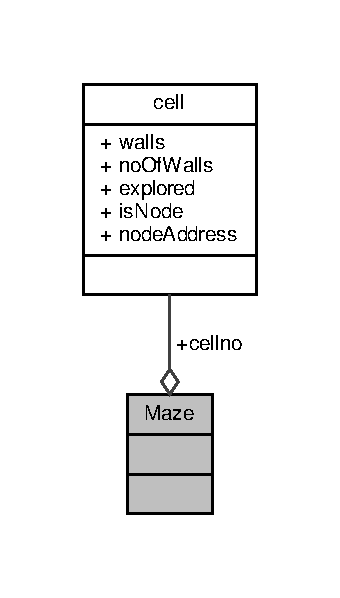
\includegraphics[width=163pt]{structMaze__coll__graph}
\end{center}
\end{figure}
\subsection*{Public Attributes}
\begin{DoxyCompactItemize}
\item 
\hyperlink{structcell}{cell} \hyperlink{structMaze_ae37dc660fb366743f092d44446bc3733}{cellno} \mbox{[}\hyperlink{MappingFunctions_8h_aed89bd71aee8be823e8a20ec4e093c1e}{H\+E\+I\+G\+HT}\mbox{]}\mbox{[}\hyperlink{MappingFunctions_8h_a241aeeb764887ae5e3de58b98f04b16d}{W\+I\+D\+TH}\mbox{]}
\end{DoxyCompactItemize}


\subsection{Detailed Description}
Contains the representation of the maze itself. 

\subsection{Member Data Documentation}
\mbox{\Hypertarget{structMaze_ae37dc660fb366743f092d44446bc3733}\label{structMaze_ae37dc660fb366743f092d44446bc3733}} 
\index{Maze@{Maze}!cellno@{cellno}}
\index{cellno@{cellno}!Maze@{Maze}}
\subsubsection{\texorpdfstring{cellno}{cellno}}
{\footnotesize\ttfamily \hyperlink{structcell}{cell} Maze\+::cellno\mbox{[}\hyperlink{MappingFunctions_8h_aed89bd71aee8be823e8a20ec4e093c1e}{H\+E\+I\+G\+HT}\mbox{]}\mbox{[}\hyperlink{MappingFunctions_8h_a241aeeb764887ae5e3de58b98f04b16d}{W\+I\+D\+TH}\mbox{]}}

Array of cells used as the maze representation 

The documentation for this struct was generated from the following file\+:\begin{DoxyCompactItemize}
\item 
Algorithm/\hyperlink{MappingFunctions_8h}{Mapping\+Functions.\+h}\end{DoxyCompactItemize}

\hypertarget{structMouse}{}\section{Mouse Struct Reference}
\label{structMouse}\index{Mouse@{Mouse}}


Representation of the \hyperlink{structMouse}{Mouse} in virtual space.  




{\ttfamily \#include $<$Map\+Maze.\+h$>$}



Collaboration diagram for Mouse\+:
\nopagebreak
\begin{figure}[H]
\begin{center}
\leavevmode
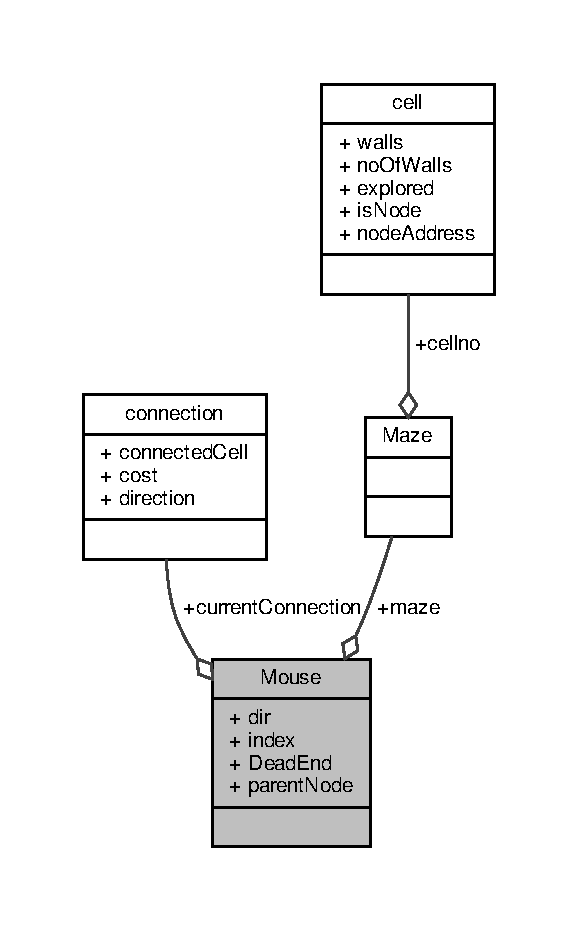
\includegraphics[width=278pt]{structMouse__coll__graph}
\end{center}
\end{figure}
\subsection*{Public Attributes}
\begin{DoxyCompactItemize}
\item 
unsigned int \hyperlink{structMouse_a6d4adc5b89ee69f33487e894e94b2640}{dir}\+: 4
\item 
unsigned char \hyperlink{structMouse_acdc68538ce06d1a8c134b359baf1ca54}{index}
\item 
unsigned int \hyperlink{structMouse_ad3d231b3da189659a15447dcb3e94fed}{Dead\+End}\+: 1
\item 
struct \hyperlink{structMaze}{Maze} $\ast$ \hyperlink{structMouse_ab8306542bdc35dfbbf53e734a364124e}{maze}
\item 
unsigned char \hyperlink{structMouse_ae6ac50ea4f691724ca55079ea4ddbd4b}{parent\+Node}
\item 
struct \hyperlink{structconnection}{connection} \hyperlink{structMouse_a63ce4210cb8aaec17760f2a0191aa42f}{current\+Connection}
\end{DoxyCompactItemize}


\subsection{Detailed Description}
Representation of the \hyperlink{structMouse}{Mouse} in virtual space. 

represents the mouse that inhabits the virtual maze. including physical attributes and debugging info. 

\subsection{Member Data Documentation}
\mbox{\Hypertarget{structMouse_a63ce4210cb8aaec17760f2a0191aa42f}\label{structMouse_a63ce4210cb8aaec17760f2a0191aa42f}} 
\index{Mouse@{Mouse}!current\+Connection@{current\+Connection}}
\index{current\+Connection@{current\+Connection}!Mouse@{Mouse}}
\subsubsection{\texorpdfstring{current\+Connection}{currentConnection}}
{\footnotesize\ttfamily struct \hyperlink{structconnection}{connection} Mouse\+::current\+Connection}

Info about current exploration from parent \hyperlink{structNode}{Node} \mbox{\Hypertarget{structMouse_ad3d231b3da189659a15447dcb3e94fed}\label{structMouse_ad3d231b3da189659a15447dcb3e94fed}} 
\index{Mouse@{Mouse}!Dead\+End@{Dead\+End}}
\index{Dead\+End@{Dead\+End}!Mouse@{Mouse}}
\subsubsection{\texorpdfstring{Dead\+End}{DeadEnd}}
{\footnotesize\ttfamily unsigned int Mouse\+::\+Dead\+End}

Marks whether backtracking from a dead end \mbox{\Hypertarget{structMouse_a6d4adc5b89ee69f33487e894e94b2640}\label{structMouse_a6d4adc5b89ee69f33487e894e94b2640}} 
\index{Mouse@{Mouse}!dir@{dir}}
\index{dir@{dir}!Mouse@{Mouse}}
\subsubsection{\texorpdfstring{dir}{dir}}
{\footnotesize\ttfamily unsigned int Mouse\+::dir}

Direction the mouse is facing \mbox{\Hypertarget{structMouse_acdc68538ce06d1a8c134b359baf1ca54}\label{structMouse_acdc68538ce06d1a8c134b359baf1ca54}} 
\index{Mouse@{Mouse}!index@{index}}
\index{index@{index}!Mouse@{Mouse}}
\subsubsection{\texorpdfstring{index}{index}}
{\footnotesize\ttfamily unsigned char Mouse\+::index}

Position of the mouse within the maze \mbox{\Hypertarget{structMouse_ab8306542bdc35dfbbf53e734a364124e}\label{structMouse_ab8306542bdc35dfbbf53e734a364124e}} 
\index{Mouse@{Mouse}!maze@{maze}}
\index{maze@{maze}!Mouse@{Mouse}}
\subsubsection{\texorpdfstring{maze}{maze}}
{\footnotesize\ttfamily struct \hyperlink{structMaze}{Maze}$\ast$ Mouse\+::maze}

contains the mouse\textquotesingle{}s model of the maze \mbox{\Hypertarget{structMouse_ae6ac50ea4f691724ca55079ea4ddbd4b}\label{structMouse_ae6ac50ea4f691724ca55079ea4ddbd4b}} 
\index{Mouse@{Mouse}!parent\+Node@{parent\+Node}}
\index{parent\+Node@{parent\+Node}!Mouse@{Mouse}}
\subsubsection{\texorpdfstring{parent\+Node}{parentNode}}
{\footnotesize\ttfamily unsigned char Mouse\+::parent\+Node}

index of \hyperlink{structNode}{Node} last viseted in nodelist, next node found will be connected to this 

The documentation for this struct was generated from the following file\+:\begin{DoxyCompactItemize}
\item 
Algorithm/Map\+Maze.\+h\end{DoxyCompactItemize}

\hypertarget{structNode}{}\section{Node Struct Reference}
\label{structNode}\index{Node@{Node}}


All info about a given \hyperlink{structNode}{Node}.  




{\ttfamily \#include $<$Mapping\+Functions.\+h$>$}



Collaboration diagram for Node\+:
\nopagebreak
\begin{figure}[H]
\begin{center}
\leavevmode
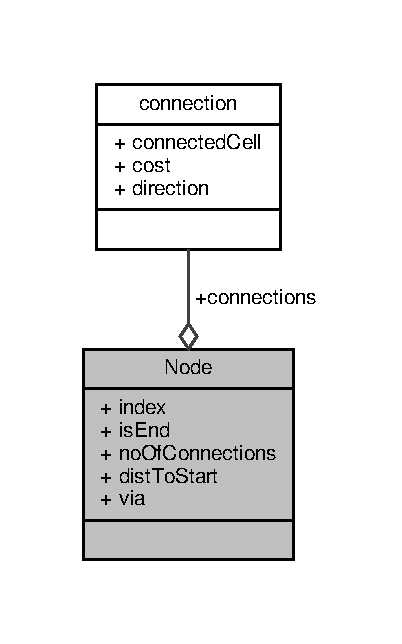
\includegraphics[width=193pt]{structNode__coll__graph}
\end{center}
\end{figure}
\subsection*{Public Attributes}
\begin{DoxyCompactItemize}
\item 
unsigned char \hyperlink{structNode_a77c45b2ff49ea5dc4195fed43e7787c2}{index}
\item 
unsigned int \hyperlink{structNode_abc8ade5cf38b553b33542473c104272a}{is\+End}\+: 1
\item 
unsigned int \hyperlink{structNode_a1ca0af175fe450a22f8d8625f0b58cbd}{no\+Of\+Connections}\+: 3
\item 
struct \hyperlink{structconnection}{connection} \hyperlink{structNode_a1552d162ffa511bd47eb78cfe89240d1}{connections} \mbox{[}4\mbox{]}
\item 
int \hyperlink{structNode_ae66c167e6d151204d510f418a81f4afc}{dist\+To\+Start}
\item 
unsigned char \hyperlink{structNode_a63fd18834461e80cc0ce292269f6f169}{via}
\end{DoxyCompactItemize}


\subsection{Detailed Description}
All info about a given \hyperlink{structNode}{Node}. 

\subsection{Member Data Documentation}
\mbox{\Hypertarget{structNode_a1552d162ffa511bd47eb78cfe89240d1}\label{structNode_a1552d162ffa511bd47eb78cfe89240d1}} 
\index{Node@{Node}!connections@{connections}}
\index{connections@{connections}!Node@{Node}}
\subsubsection{\texorpdfstring{connections}{connections}}
{\footnotesize\ttfamily struct \hyperlink{structconnection}{connection} Node\+::connections\mbox{[}4\mbox{]}}

Array of connected nodes \mbox{\Hypertarget{structNode_ae66c167e6d151204d510f418a81f4afc}\label{structNode_ae66c167e6d151204d510f418a81f4afc}} 
\index{Node@{Node}!dist\+To\+Start@{dist\+To\+Start}}
\index{dist\+To\+Start@{dist\+To\+Start}!Node@{Node}}
\subsubsection{\texorpdfstring{dist\+To\+Start}{distToStart}}
{\footnotesize\ttfamily int Node\+::dist\+To\+Start}

Shortest distance found to centre of maze. -\/1 represents infinite distance \mbox{\Hypertarget{structNode_a77c45b2ff49ea5dc4195fed43e7787c2}\label{structNode_a77c45b2ff49ea5dc4195fed43e7787c2}} 
\index{Node@{Node}!index@{index}}
\index{index@{index}!Node@{Node}}
\subsubsection{\texorpdfstring{index}{index}}
{\footnotesize\ttfamily unsigned char Node\+::index}

index of the cell that this node references \mbox{\Hypertarget{structNode_abc8ade5cf38b553b33542473c104272a}\label{structNode_abc8ade5cf38b553b33542473c104272a}} 
\index{Node@{Node}!is\+End@{is\+End}}
\index{is\+End@{is\+End}!Node@{Node}}
\subsubsection{\texorpdfstring{is\+End}{isEnd}}
{\footnotesize\ttfamily unsigned int Node\+::is\+End}

Marks whether the \hyperlink{structNode}{Node} is at the centre of the maze \mbox{\Hypertarget{structNode_a1ca0af175fe450a22f8d8625f0b58cbd}\label{structNode_a1ca0af175fe450a22f8d8625f0b58cbd}} 
\index{Node@{Node}!no\+Of\+Connections@{no\+Of\+Connections}}
\index{no\+Of\+Connections@{no\+Of\+Connections}!Node@{Node}}
\subsubsection{\texorpdfstring{no\+Of\+Connections}{noOfConnections}}
{\footnotesize\ttfamily unsigned int Node\+::no\+Of\+Connections}

Number of Nodes connected to this one \mbox{\Hypertarget{structNode_a63fd18834461e80cc0ce292269f6f169}\label{structNode_a63fd18834461e80cc0ce292269f6f169}} 
\index{Node@{Node}!via@{via}}
\index{via@{via}!Node@{Node}}
\subsubsection{\texorpdfstring{via}{via}}
{\footnotesize\ttfamily unsigned char Node\+::via}

\hyperlink{structNode}{Node} shortest route goes through to get here. 

The documentation for this struct was generated from the following file\+:\begin{DoxyCompactItemize}
\item 
Algorithm/\hyperlink{MappingFunctions_8h}{Mapping\+Functions.\+h}\end{DoxyCompactItemize}

\hypertarget{structStack}{}\section{Stack Struct Reference}
\label{structStack}\index{Stack@{Stack}}


array of data that is the \hyperlink{structStack}{Stack}.  




{\ttfamily \#include $<$Stacks.\+h$>$}



Collaboration diagram for Stack\+:
\nopagebreak
\begin{figure}[H]
\begin{center}
\leavevmode
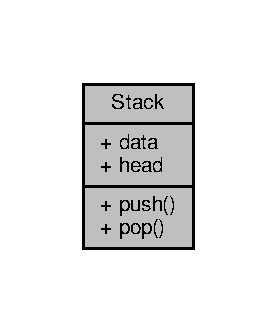
\includegraphics[width=133pt]{structStack__coll__graph}
\end{center}
\end{figure}
\subsection*{Public Member Functions}
\begin{DoxyCompactItemize}
\item 
void \hyperlink{structStack_a0bd90a5dfacc09f2df0382c269e0236b}{push} (\hyperlink{structStack}{Stack} $\ast$stack, unsigned char Newdata)
\begin{DoxyCompactList}\small\item\em pushes item onto a stack. \end{DoxyCompactList}\item 
unsigned char \hyperlink{structStack_aa2c179f9f71cccf23778012d4e9326de}{pop} (\hyperlink{structStack}{Stack} $\ast$stack)
\begin{DoxyCompactList}\small\item\em pops an item from the top of the stack. \end{DoxyCompactList}\end{DoxyCompactItemize}
\subsection*{Public Attributes}
\begin{DoxyCompactItemize}
\item 
unsigned char \hyperlink{structStack_af7c19f315867ae89b59eb06bb1e6c8bf}{data} \mbox{[}\hyperlink{MappingFunctions_8h_a241aeeb764887ae5e3de58b98f04b16d}{W\+I\+D\+TH} $\ast$\hyperlink{MappingFunctions_8h_aed89bd71aee8be823e8a20ec4e093c1e}{H\+E\+I\+G\+HT} $\ast$2\mbox{]}
\item 
unsigned char \hyperlink{structStack_ae9de4145f4aee2664247e585ec86d220}{head}
\end{DoxyCompactItemize}


\subsection{Detailed Description}
array of data that is the \hyperlink{structStack}{Stack}. 

The size of the stack equal to number of cells in the maze. 

\subsection{Member Function Documentation}
\mbox{\Hypertarget{structStack_aa2c179f9f71cccf23778012d4e9326de}\label{structStack_aa2c179f9f71cccf23778012d4e9326de}} 
\index{Stack@{Stack}!pop@{pop}}
\index{pop@{pop}!Stack@{Stack}}
\subsubsection{\texorpdfstring{pop()}{pop()}}
{\footnotesize\ttfamily unsigned char pop (\begin{DoxyParamCaption}\item[{\hyperlink{structStack}{Stack} $\ast$}]{stack }\end{DoxyParamCaption})}



pops an item from the top of the stack. 

returns the data from the top-\/most stackitem, points the stack pointer to the item below where it was and frees the topmost item.


\begin{DoxyParams}{Parameters}
{\em stack} & the stack from which the data will be popped. \\
\hline
\end{DoxyParams}
\mbox{\Hypertarget{structStack_a0bd90a5dfacc09f2df0382c269e0236b}\label{structStack_a0bd90a5dfacc09f2df0382c269e0236b}} 
\index{Stack@{Stack}!push@{push}}
\index{push@{push}!Stack@{Stack}}
\subsubsection{\texorpdfstring{push()}{push()}}
{\footnotesize\ttfamily void push (\begin{DoxyParamCaption}\item[{\hyperlink{structStack}{Stack} $\ast$}]{stack,  }\item[{unsigned char}]{Newdata }\end{DoxyParamCaption})}



pushes item onto a stack. 

creates a new stackitem which contains the new data and points to the current head of the stack. The stack pointer is then moved to point at the new stackitem.


\begin{DoxyParams}{Parameters}
{\em stack} & the stack that the data will be pushed to. \\
\hline
{\em Newdata} & the data that will be pushed to the stack. \\
\hline
\end{DoxyParams}


\subsection{Member Data Documentation}
\mbox{\Hypertarget{structStack_af7c19f315867ae89b59eb06bb1e6c8bf}\label{structStack_af7c19f315867ae89b59eb06bb1e6c8bf}} 
\index{Stack@{Stack}!data@{data}}
\index{data@{data}!Stack@{Stack}}
\subsubsection{\texorpdfstring{data}{data}}
{\footnotesize\ttfamily unsigned char Stack\+::data\mbox{[}\hyperlink{MappingFunctions_8h_a241aeeb764887ae5e3de58b98f04b16d}{W\+I\+D\+TH} $\ast$\hyperlink{MappingFunctions_8h_aed89bd71aee8be823e8a20ec4e093c1e}{H\+E\+I\+G\+HT} $\ast$2\mbox{]}}

data that is stored in the \hyperlink{structStack}{Stack} \mbox{\Hypertarget{structStack_ae9de4145f4aee2664247e585ec86d220}\label{structStack_ae9de4145f4aee2664247e585ec86d220}} 
\index{Stack@{Stack}!head@{head}}
\index{head@{head}!Stack@{Stack}}
\subsubsection{\texorpdfstring{head}{head}}
{\footnotesize\ttfamily unsigned char Stack\+::head}

head of the \hyperlink{structStack}{Stack} where data is pushed to and popped from 

The documentation for this struct was generated from the following file\+:\begin{DoxyCompactItemize}
\item 
\hyperlink{Stacks_8h}{Stacks.\+h}\end{DoxyCompactItemize}

\chapter{File Documentation}
\hypertarget{Dijekstra_8h}{}\section{Algorithm/\+Dijekstra.h File Reference}
\label{Dijekstra_8h}\index{Algorithm/\+Dijekstra.\+h@{Algorithm/\+Dijekstra.\+h}}


dijekstra\textquotesingle{}s function and cocktail sort.  


{\ttfamily \#include \char`\"{}Mapping\+Functions.\+h\char`\"{}}\newline
Include dependency graph for Dijekstra.\+h\+:
\nopagebreak
\begin{figure}[H]
\begin{center}
\leavevmode
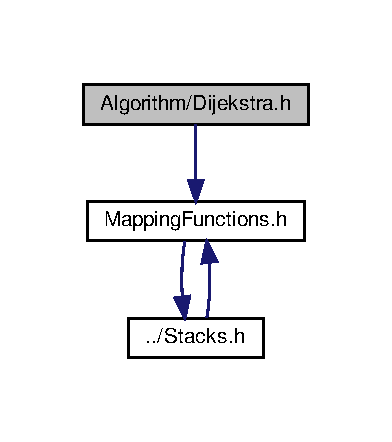
\includegraphics[width=188pt]{Dijekstra_8h__incl}
\end{center}
\end{figure}
This graph shows which files directly or indirectly include this file\+:
\nopagebreak
\begin{figure}[H]
\begin{center}
\leavevmode
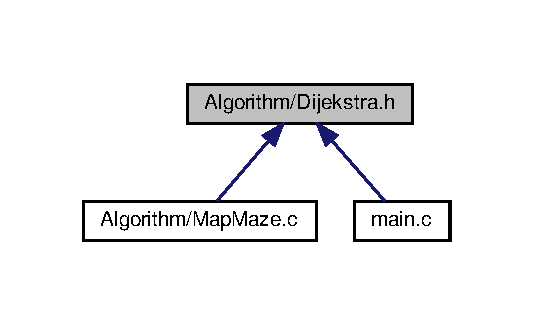
\includegraphics[width=256pt]{Dijekstra_8h__dep__incl}
\end{center}
\end{figure}
\subsection*{Functions}
\begin{DoxyCompactItemize}
\item 
\hyperlink{structStack}{Stack} \hyperlink{Dijekstra_8h_ae4cdc18ed3a8514e0412e0d455f8feeb}{dijekstra} (struct \hyperlink{structMaze}{Maze} $\ast$maze, \hyperlink{structNode}{Node} nodemap\mbox{[}\hyperlink{MappingFunctions_8h_abd2aacdca9cb2a1a30f3392256b96ea3}{M\+A\+X\+\_\+\+N\+O\+D\+ES}\mbox{]}, \hyperlink{structNode}{Node} $\ast$start, \hyperlink{structNode}{Node} $\ast$end, char startdir)
\begin{DoxyCompactList}\small\item\em Find fastest route between 2 Nodes. \end{DoxyCompactList}\item 
void \hyperlink{Dijekstra_8h_a6fa19831b9a69465e0810ca738d984c2}{cocktail} (\hyperlink{structNode}{Node} $\ast$arr\mbox{[}\hyperlink{MappingFunctions_8h_abd2aacdca9cb2a1a30f3392256b96ea3}{M\+A\+X\+\_\+\+N\+O\+D\+ES}\mbox{]})
\begin{DoxyCompactList}\small\item\em cocktail sorts given array. \end{DoxyCompactList}\end{DoxyCompactItemize}


\subsection{Detailed Description}
dijekstra\textquotesingle{}s function and cocktail sort. 

Cocktail sort is used to order the priority queue after each time a \hyperlink{structNode}{Node} has finished being checked by the dijekstra\textquotesingle{}s function.

\begin{DoxyAuthor}{Author}
Nick Appleton @ U\+WE Robotics
\end{DoxyAuthor}
\begin{DoxyDate}{Date}
16/3/19 
\end{DoxyDate}


\subsection{Function Documentation}
\mbox{\Hypertarget{Dijekstra_8h_a6fa19831b9a69465e0810ca738d984c2}\label{Dijekstra_8h_a6fa19831b9a69465e0810ca738d984c2}} 
\index{Dijekstra.\+h@{Dijekstra.\+h}!cocktail@{cocktail}}
\index{cocktail@{cocktail}!Dijekstra.\+h@{Dijekstra.\+h}}
\subsubsection{\texorpdfstring{cocktail()}{cocktail()}}
{\footnotesize\ttfamily void cocktail (\begin{DoxyParamCaption}\item[{\hyperlink{structNode}{Node} $\ast$}]{arr\mbox{[}\+M\+A\+X\+\_\+\+N\+O\+D\+E\+S\mbox{]} }\end{DoxyParamCaption})}



cocktail sorts given array. 


\begin{DoxyParams}{Parameters}
{\em arr} & array to be sorted \\
\hline
\end{DoxyParams}
\mbox{\Hypertarget{Dijekstra_8h_ae4cdc18ed3a8514e0412e0d455f8feeb}\label{Dijekstra_8h_ae4cdc18ed3a8514e0412e0d455f8feeb}} 
\index{Dijekstra.\+h@{Dijekstra.\+h}!dijekstra@{dijekstra}}
\index{dijekstra@{dijekstra}!Dijekstra.\+h@{Dijekstra.\+h}}
\subsubsection{\texorpdfstring{dijekstra()}{dijekstra()}}
{\footnotesize\ttfamily \hyperlink{structStack}{Stack} dijekstra (\begin{DoxyParamCaption}\item[{struct \hyperlink{structMaze}{Maze} $\ast$}]{maze,  }\item[{\hyperlink{structNode}{Node}}]{nodemap\mbox{[}\+M\+A\+X\+\_\+\+N\+O\+D\+E\+S\mbox{]},  }\item[{\hyperlink{structNode}{Node} $\ast$}]{start,  }\item[{\hyperlink{structNode}{Node} $\ast$}]{end,  }\item[{char}]{startdir }\end{DoxyParamCaption})}



Find fastest route between 2 Nodes. 

Uses dijekstra\textquotesingle{}s algorithm to find the shortest route thorugh the Nodemap. It routes through the maze, pushing each move that needs to be made to a stack. This stack is then returned.

The stack\textquotesingle{}s format is\+: initial on-\/the-\/spot turn to face the correct direction, then it has the initial forward move (or 0 if there isn\textquotesingle{}t one). From there it alternates between each forward move and each turn required to get into the next cell. The turns include the move into the Next cell. Last item in stack is a straight, moves into the end \hyperlink{structNode}{Node} cell.


\begin{DoxyParams}{Parameters}
{\em maze} & maze to search through \\
\hline
{\em nodemap} & nodemap of the maze given \\
\hline
{\em start} & location of the \hyperlink{structNode}{Node} to start from \\
\hline
{\em end} & location of the \hyperlink{structNode}{Node} to get to \\
\hline
{\em startdir} & direction the mouse is facing at the start \\
\hline
\end{DoxyParams}
\begin{DoxyReturn}{Returns}
satck of moves to get from start to finish 
\end{DoxyReturn}

\hypertarget{MapMaze_8c}{}\section{Algorithm/\+Map\+Maze.c File Reference}
\label{MapMaze_8c}\index{Algorithm/\+Map\+Maze.\+c@{Algorithm/\+Map\+Maze.\+c}}


Fully maps the maze.  


{\ttfamily \#include \char`\"{}simulator.\+h\char`\"{}}\newline
{\ttfamily \#include \char`\"{}Map\+Maze.\+h\char`\"{}}\newline
{\ttfamily \#include \char`\"{}Dijekstra.\+h\char`\"{}}\newline
{\ttfamily \#include $<$stdlib.\+h$>$}\newline
{\ttfamily \#include $<$stdio.\+h$>$}\newline
Include dependency graph for Map\+Maze.\+c\+:
\nopagebreak
\begin{figure}[H]
\begin{center}
\leavevmode
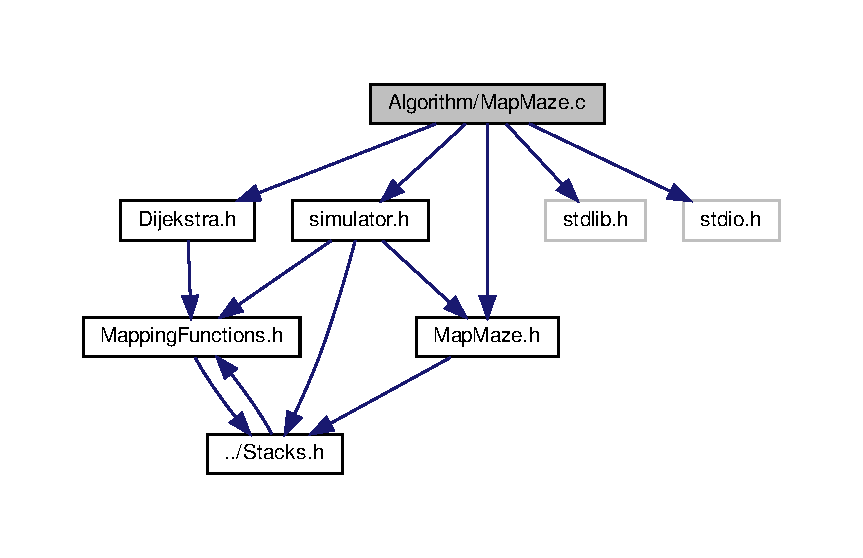
\includegraphics[width=350pt]{MapMaze_8c__incl}
\end{center}
\end{figure}
\subsection*{Macros}
\textbf{ }\par
\begin{DoxyCompactItemize}
\item 
\#define \hyperlink{MapMaze_8c_ad8a5d8c4e3342fb668142df792e93f38}{S\+I\+M\+U\+L\+A\+T\+OR}~1
\begin{DoxyCompactList}\small\item\em Use simulator or \hyperlink{structMouse}{Mouse}. \end{DoxyCompactList}\end{DoxyCompactItemize}

\subsection*{Functions}
\begin{DoxyCompactItemize}
\item 
void \hyperlink{MapMaze_8c_a56582780c29894e5424db2aa1eb5ee20}{mapmaze} (struct \hyperlink{structMaze}{Maze} $\ast$maze\+Arg, \hyperlink{structNode}{Node} $\ast$nodelist)
\begin{DoxyCompactList}\small\item\em main maze-\/mapping function. \end{DoxyCompactList}\item 
void \hyperlink{MapMaze_8c_ac2634689289c7d3e68fcbe252e5cc7f3}{Setup\+Mapping} (\hyperlink{structStack}{Stack} $\ast$openlist, \hyperlink{structNode}{Node} $\ast$nodelist)
\begin{DoxyCompactList}\small\item\em sets up the mouse ready to map out the maze. \end{DoxyCompactList}\item 
unsigned char \hyperlink{MapMaze_8c_a986e541ab618881448b4b0598b56231f}{create\+Node} (unsigned char index, \hyperlink{structNode}{Node} $\ast$nodelist)
\begin{DoxyCompactList}\small\item\em creates a new node. \end{DoxyCompactList}\item 
void \hyperlink{MapMaze_8c_a6d8e855069513377f892eb0df781ba1e}{checkcurrentcell} (\hyperlink{structStack}{Stack} $\ast$openlist, \hyperlink{structNode}{Node} $\ast$nodelist, \hyperlink{structStack}{Stack} $\ast$history)
\begin{DoxyCompactList}\small\item\em updates info on the cell currently occupied. \end{DoxyCompactList}\item 
void \hyperlink{MapMaze_8c_a4ddfd0bcc7e064d6a5093be6a3911cc9}{Connect\+Nodes} (\hyperlink{structNode}{Node} $\ast$nodelist, unsigned char dir)
\begin{DoxyCompactList}\small\item\em Connects the parent node to the current cell. \end{DoxyCompactList}\item 
void \hyperlink{MapMaze_8c_a44cea4dfa361e85c137fb8acf0a7687f}{Explore\+New\+Cell} (\hyperlink{structStack}{Stack} $\ast$openlist, \hyperlink{structStack}{Stack} $\ast$history, \hyperlink{structNode}{Node} $\ast$nodelist)
\begin{DoxyCompactList}\small\item\em Used to get to new areas. \end{DoxyCompactList}\item 
unsigned char \hyperlink{MapMaze_8c_a3b66563016c1681b10fc776de488ad79}{identify\+Direction} (unsigned char target)
\begin{DoxyCompactList}\small\item\em identify in which direction a cell is. \end{DoxyCompactList}\item 
void \hyperlink{MapMaze_8c_a2e0744c820e2dfb79f035fc4ab09517e}{move\+To\+Adjacent\+Cell} (unsigned char direction)
\begin{DoxyCompactList}\small\item\em move mouse into an adjacent cell in the direction given. \end{DoxyCompactList}\item 
void \hyperlink{MapMaze_8c_a53ecd9bd5b6f7445b0e66e89e3263178}{virtual\+Mouse} (\hyperlink{structNode}{Node} $\ast$nodelist)
\begin{DoxyCompactList}\small\item\em corrects any known but unexplored dead-\/ends. \end{DoxyCompactList}\item 
void \hyperlink{MapMaze_8c_a960e470045bed71f16ce4ff8a6614f0b}{V\+Mcheck} (unsigned char index, \hyperlink{structNode}{Node} $\ast$nodelist)
\begin{DoxyCompactList}\small\item\em checks one cell for dead end and corrects it. \end{DoxyCompactList}\item 
void \hyperlink{MapMaze_8c_a1edcad7e629303c8f8a47ce88a69463f}{Destroy\+Node} (\hyperlink{structNode}{Node} $\ast$nodelist, unsigned char index)
\begin{DoxyCompactList}\small\item\em destroy a given \hyperlink{structNode}{Node}. \end{DoxyCompactList}\end{DoxyCompactItemize}
\subsection*{Variables}
\begin{DoxyCompactItemize}
\item 
\mbox{\Hypertarget{MapMaze_8c_a07faa847230d0abd8c3db00e3f8cae7a}\label{MapMaze_8c_a07faa847230d0abd8c3db00e3f8cae7a}} 
\hyperlink{structMouse}{Mouse} \hyperlink{MapMaze_8c_a07faa847230d0abd8c3db00e3f8cae7a}{mouse}
\begin{DoxyCompactList}\small\item\em global representation of the mouse used by every function. \end{DoxyCompactList}\end{DoxyCompactItemize}


\subsection{Detailed Description}
Fully maps the maze. 

Maps the full maze including placing nodes and finding the connections between those Nodes.

\begin{DoxyAuthor}{Author}
Nick Appleton @ U\+WE Robotics
\end{DoxyAuthor}
\begin{DoxyDate}{Date}
24/2/19 
\end{DoxyDate}


\subsection{Macro Definition Documentation}
\mbox{\Hypertarget{MapMaze_8c_ad8a5d8c4e3342fb668142df792e93f38}\label{MapMaze_8c_ad8a5d8c4e3342fb668142df792e93f38}} 
\index{Map\+Maze.\+c@{Map\+Maze.\+c}!S\+I\+M\+U\+L\+A\+T\+OR@{S\+I\+M\+U\+L\+A\+T\+OR}}
\index{S\+I\+M\+U\+L\+A\+T\+OR@{S\+I\+M\+U\+L\+A\+T\+OR}!Map\+Maze.\+c@{Map\+Maze.\+c}}
\subsubsection{\texorpdfstring{S\+I\+M\+U\+L\+A\+T\+OR}{SIMULATOR}}
{\footnotesize\ttfamily \#define S\+I\+M\+U\+L\+A\+T\+OR~1}



Use simulator or \hyperlink{structMouse}{Mouse}. 

If the variable is set to 1, the simulator will be used. Otherwise the target will be the actual mouse. 

\subsection{Function Documentation}
\mbox{\Hypertarget{MapMaze_8c_a6d8e855069513377f892eb0df781ba1e}\label{MapMaze_8c_a6d8e855069513377f892eb0df781ba1e}} 
\index{Map\+Maze.\+c@{Map\+Maze.\+c}!checkcurrentcell@{checkcurrentcell}}
\index{checkcurrentcell@{checkcurrentcell}!Map\+Maze.\+c@{Map\+Maze.\+c}}
\subsubsection{\texorpdfstring{checkcurrentcell()}{checkcurrentcell()}}
{\footnotesize\ttfamily void checkcurrentcell (\begin{DoxyParamCaption}\item[{\hyperlink{structStack}{Stack} $\ast$}]{openlist,  }\item[{\hyperlink{structNode}{Node} $\ast$}]{nodelist,  }\item[{\hyperlink{structStack}{Stack} $\ast$}]{history }\end{DoxyParamCaption})}



updates info on the cell currently occupied. 

This includes correcting all the walls in the current cell and all adjacent cells, adding unexplored adjacent cells to the openlist and changing the cells properties to reflect it\textquotesingle{}s status (it\textquotesingle{}s now been explored).


\begin{DoxyImageNoCaption}
  \mbox{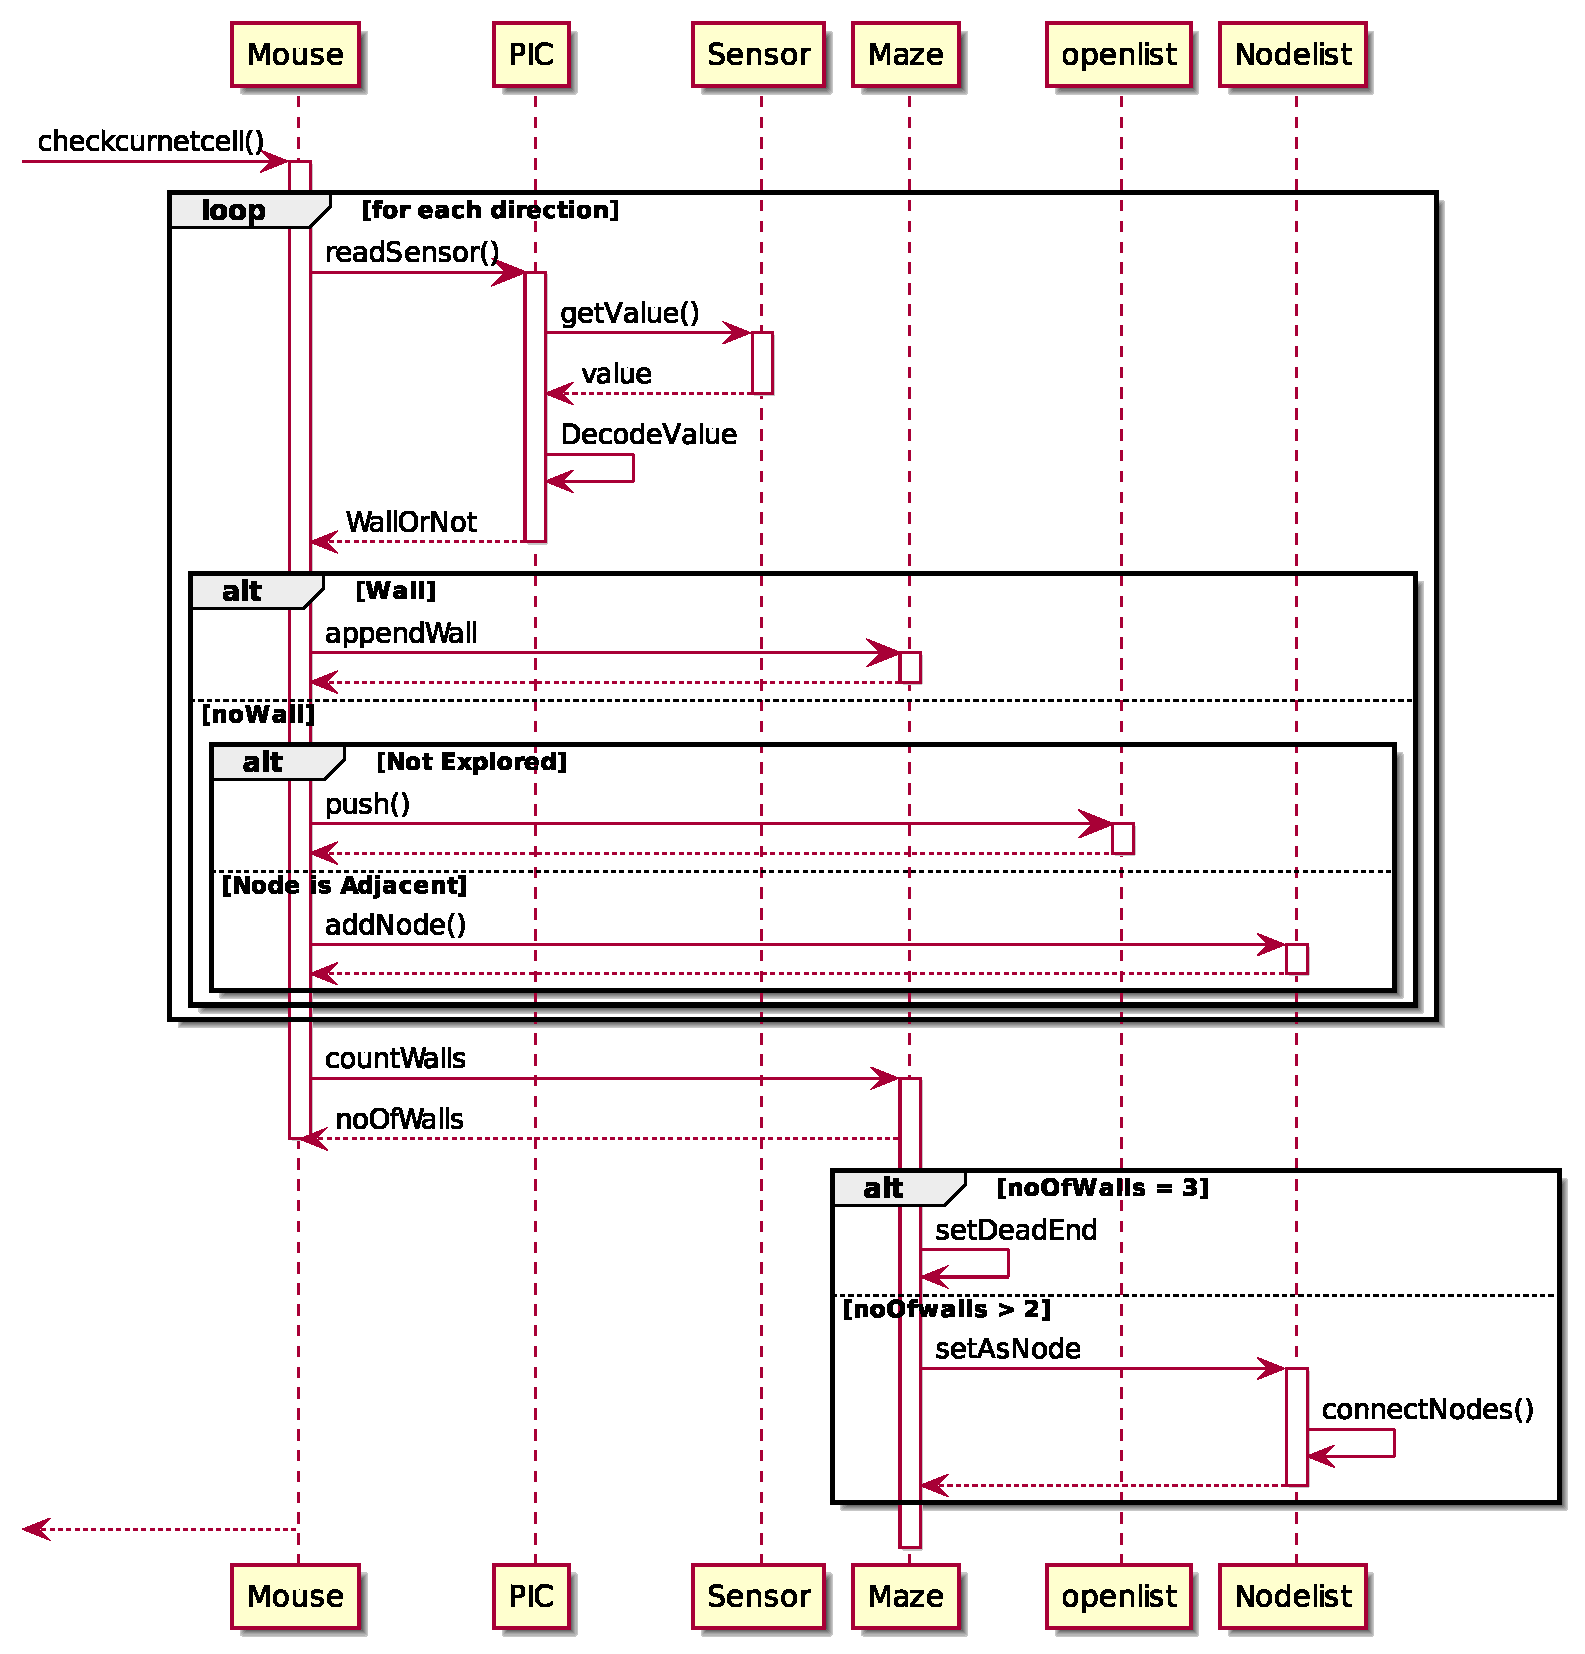
\includegraphics[width=\textwidth,height=\textheight/2,keepaspectratio=true]{inline_umlgraph_2}}
\end{DoxyImageNoCaption}



\begin{DoxyParams}{Parameters}
{\em openlist} & The stack of cells to be explored. \\
\hline
{\em nodelist} & list of all the Nodes in the maze. \\
\hline
{\em history} & stack of the cells which were visited by the mouse. \\
\hline
\end{DoxyParams}
\mbox{\Hypertarget{MapMaze_8c_a4ddfd0bcc7e064d6a5093be6a3911cc9}\label{MapMaze_8c_a4ddfd0bcc7e064d6a5093be6a3911cc9}} 
\index{Map\+Maze.\+c@{Map\+Maze.\+c}!Connect\+Nodes@{Connect\+Nodes}}
\index{Connect\+Nodes@{Connect\+Nodes}!Map\+Maze.\+c@{Map\+Maze.\+c}}
\subsubsection{\texorpdfstring{Connect\+Nodes()}{ConnectNodes()}}
{\footnotesize\ttfamily void Connect\+Nodes (\begin{DoxyParamCaption}\item[{\hyperlink{structNode}{Node} $\ast$}]{nodelist,  }\item[{unsigned char}]{dir }\end{DoxyParamCaption})}



Connects the parent node to the current cell. 

Adds a connection to the parent \hyperlink{structNode}{Node} to the current cell, also adds the connection back from current cell to parent \hyperlink{structNode}{Node}. If the current cell is not a \hyperlink{structNode}{Node}, it creates a new node to use.


\begin{DoxyParams}{Parameters}
{\em nodelist} & List of all the Nodes in the maze. \\
\hline
{\em dir} & direction in which the mouse entered the cell to be connected to the parent. \\
\hline
\end{DoxyParams}
\mbox{\Hypertarget{MapMaze_8c_a986e541ab618881448b4b0598b56231f}\label{MapMaze_8c_a986e541ab618881448b4b0598b56231f}} 
\index{Map\+Maze.\+c@{Map\+Maze.\+c}!create\+Node@{create\+Node}}
\index{create\+Node@{create\+Node}!Map\+Maze.\+c@{Map\+Maze.\+c}}
\subsubsection{\texorpdfstring{create\+Node()}{createNode()}}
{\footnotesize\ttfamily unsigned char create\+Node (\begin{DoxyParamCaption}\item[{unsigned char}]{index,  }\item[{\hyperlink{structNode}{Node} $\ast$}]{nodelist }\end{DoxyParamCaption})}



creates a new node. 

Initialises all the \hyperlink{structNode}{Node} variables, sets the cell at the correct index to a node and adds a pointer to the new node.


\begin{DoxyParams}{Parameters}
{\em index} & index at which the new \hyperlink{structNode}{Node} is to be created. \\
\hline
{\em nodelist} & List of all the Nodes in the maze. \\
\hline
\end{DoxyParams}
\begin{DoxyReturn}{Returns}
a pointer to the newly created node. 
\end{DoxyReturn}
\mbox{\Hypertarget{MapMaze_8c_a1edcad7e629303c8f8a47ce88a69463f}\label{MapMaze_8c_a1edcad7e629303c8f8a47ce88a69463f}} 
\index{Map\+Maze.\+c@{Map\+Maze.\+c}!Destroy\+Node@{Destroy\+Node}}
\index{Destroy\+Node@{Destroy\+Node}!Map\+Maze.\+c@{Map\+Maze.\+c}}
\subsubsection{\texorpdfstring{Destroy\+Node()}{DestroyNode()}}
{\footnotesize\ttfamily void Destroy\+Node (\begin{DoxyParamCaption}\item[{\hyperlink{structNode}{Node} $\ast$}]{nodelist,  }\item[{unsigned char}]{index }\end{DoxyParamCaption})}



destroy a given \hyperlink{structNode}{Node}. 

Removes \hyperlink{structNode}{Node} from nodelist by setting the distance\+To\+Start as 0.


\begin{DoxyParams}{Parameters}
{\em nodelist} & List of all Nodes in the maze. \\
\hline
{\em index} & index where the \hyperlink{structNode}{Node} to be destroyed is. \\
\hline
\end{DoxyParams}
\mbox{\Hypertarget{MapMaze_8c_a44cea4dfa361e85c137fb8acf0a7687f}\label{MapMaze_8c_a44cea4dfa361e85c137fb8acf0a7687f}} 
\index{Map\+Maze.\+c@{Map\+Maze.\+c}!Explore\+New\+Cell@{Explore\+New\+Cell}}
\index{Explore\+New\+Cell@{Explore\+New\+Cell}!Map\+Maze.\+c@{Map\+Maze.\+c}}
\subsubsection{\texorpdfstring{Explore\+New\+Cell()}{ExploreNewCell()}}
{\footnotesize\ttfamily void Explore\+New\+Cell (\begin{DoxyParamCaption}\item[{\hyperlink{structStack}{Stack} $\ast$}]{openlist,  }\item[{\hyperlink{structStack}{Stack} $\ast$}]{history,  }\item[{\hyperlink{structNode}{Node} $\ast$}]{nodelist }\end{DoxyParamCaption})}



Used to get to new areas. 

Pops the first item from the openlist and explores the cell at that index. If the cell is not accessible from the current cell, then it backtracks until it finds it.


\begin{DoxyImageNoCaption}
  \mbox{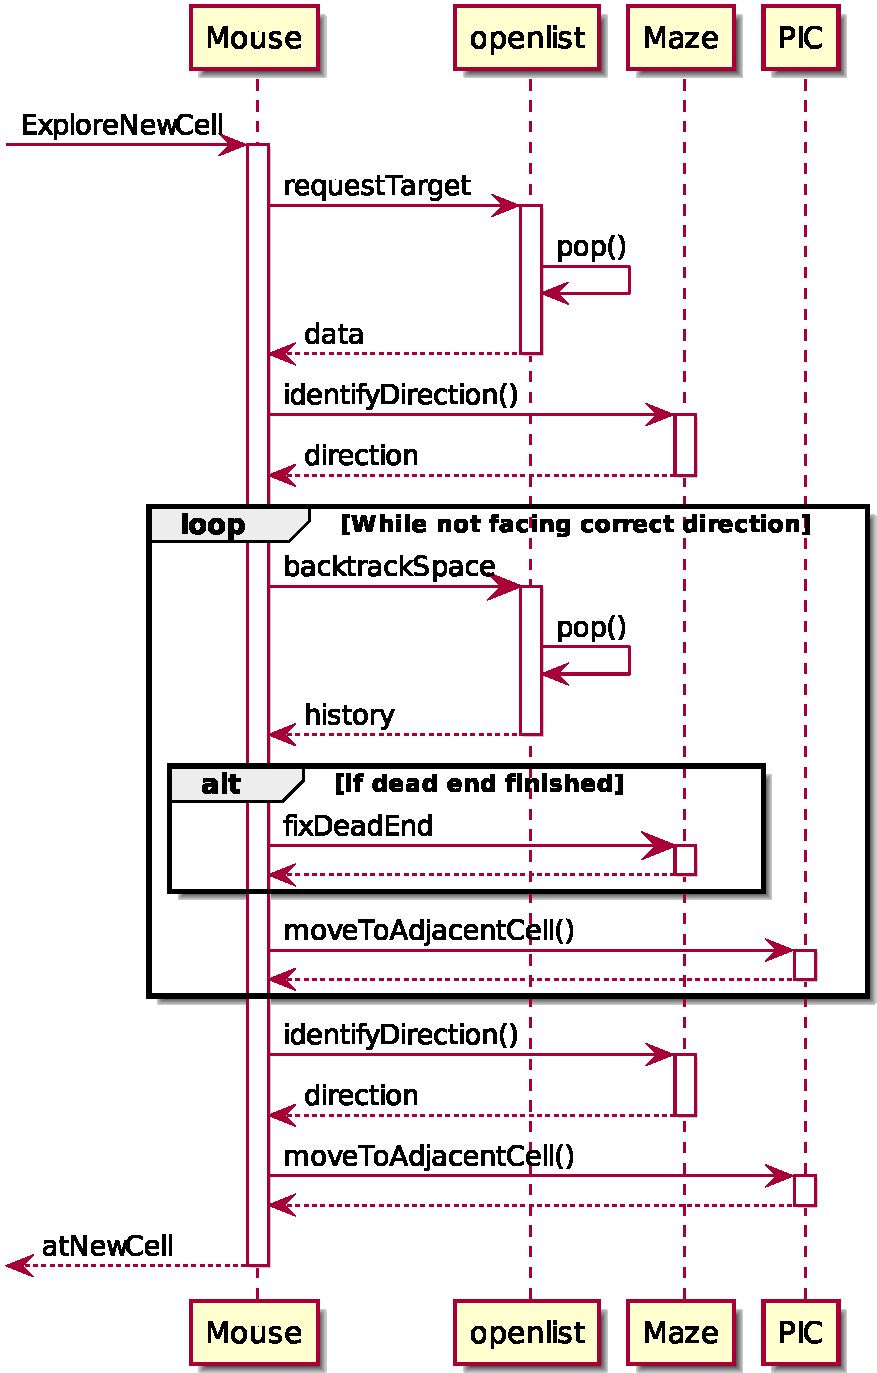
\includegraphics[width=\textwidth,height=\textheight/2,keepaspectratio=true]{inline_umlgraph_4}}
\end{DoxyImageNoCaption}



\begin{DoxyParams}{Parameters}
{\em openlist} & The stack of cells to be explored. \\
\hline
{\em history} & stack of all the places visited by the mouse \\
\hline
{\em nodelist} & List of all the Nodes in the maze. \\
\hline
\end{DoxyParams}
\mbox{\Hypertarget{MapMaze_8c_a3b66563016c1681b10fc776de488ad79}\label{MapMaze_8c_a3b66563016c1681b10fc776de488ad79}} 
\index{Map\+Maze.\+c@{Map\+Maze.\+c}!identify\+Direction@{identify\+Direction}}
\index{identify\+Direction@{identify\+Direction}!Map\+Maze.\+c@{Map\+Maze.\+c}}
\subsubsection{\texorpdfstring{identify\+Direction()}{identifyDirection()}}
{\footnotesize\ttfamily unsigned char identify\+Direction (\begin{DoxyParamCaption}\item[{unsigned char}]{target }\end{DoxyParamCaption})}



identify in which direction a cell is. 

Identifies which direction an adjacent cell is in, if the target cell is not adjacent, then 0 is returned.


\begin{DoxyParams}{Parameters}
{\em target} & the cell that the mouse is trying to get to. \\
\hline
\end{DoxyParams}
\begin{DoxyReturn}{Returns}
the direction of the adjacent cell. 
\end{DoxyReturn}
\mbox{\Hypertarget{MapMaze_8c_a56582780c29894e5424db2aa1eb5ee20}\label{MapMaze_8c_a56582780c29894e5424db2aa1eb5ee20}} 
\index{Map\+Maze.\+c@{Map\+Maze.\+c}!mapmaze@{mapmaze}}
\index{mapmaze@{mapmaze}!Map\+Maze.\+c@{Map\+Maze.\+c}}
\subsubsection{\texorpdfstring{mapmaze()}{mapmaze()}}
{\footnotesize\ttfamily void mapmaze (\begin{DoxyParamCaption}\item[{struct \hyperlink{structMaze}{Maze} $\ast$}]{maze\+Arg,  }\item[{\hyperlink{structNode}{Node} $\ast$}]{nodelist }\end{DoxyParamCaption})}



main maze-\/mapping function. 

calls all the other functions to map out the whole reachable maze.


\begin{DoxyImageNoCaption}
  \mbox{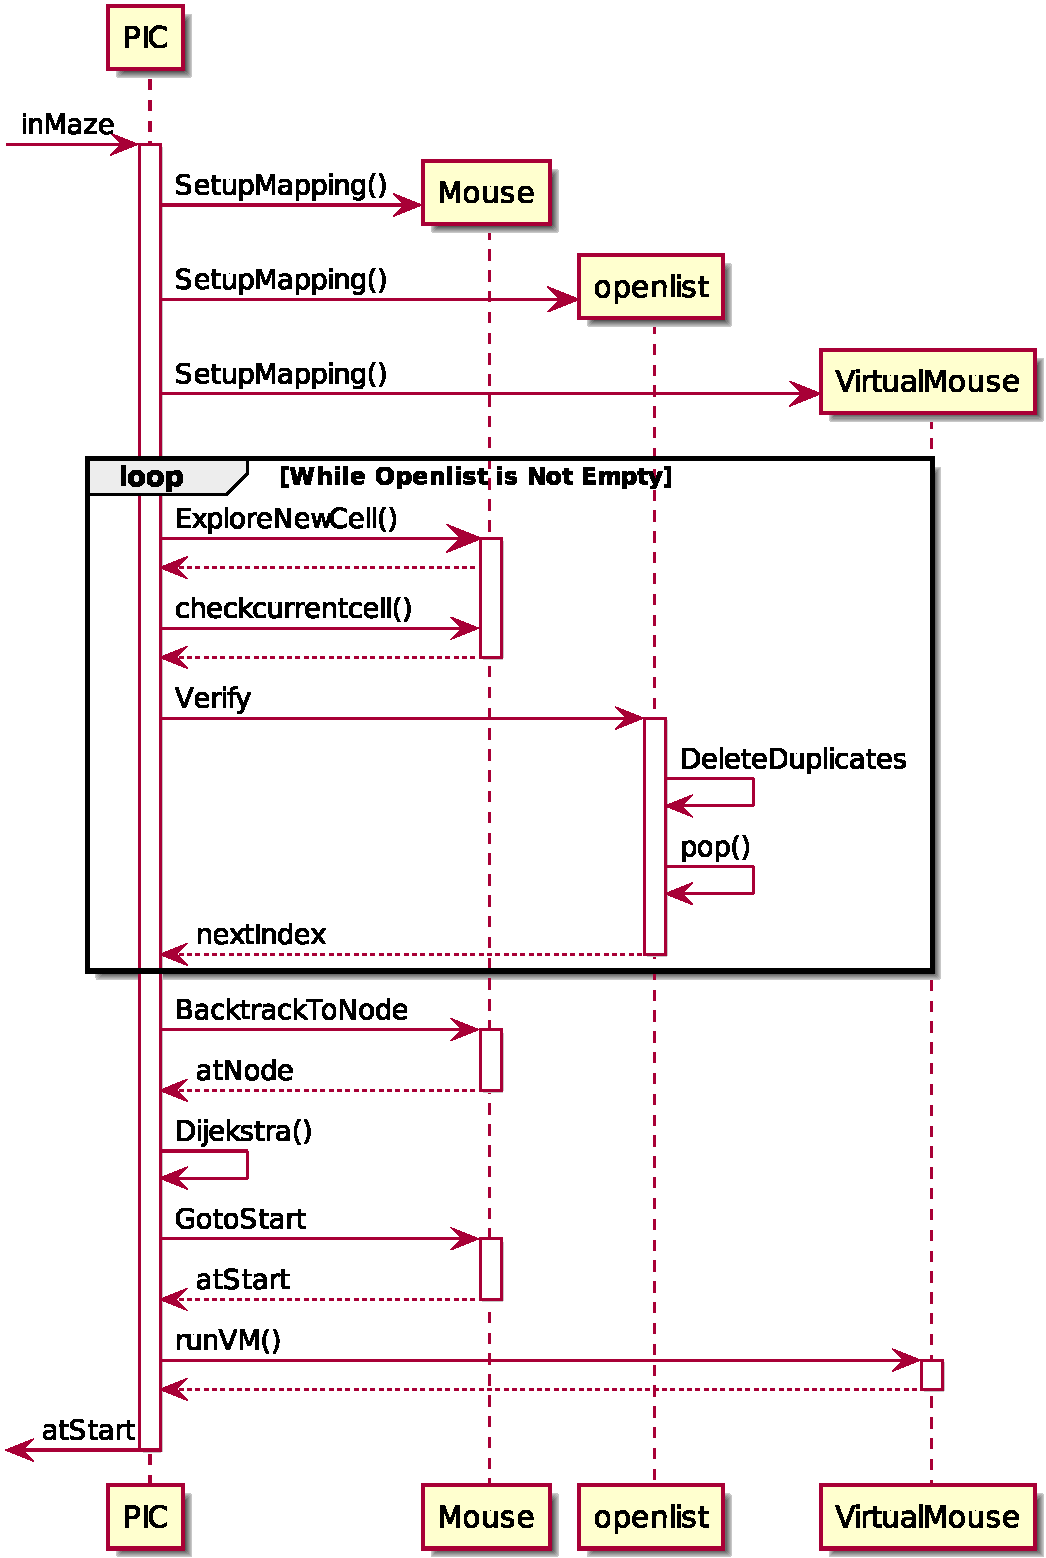
\includegraphics[width=\textwidth,height=\textheight/2,keepaspectratio=true]{inline_umlgraph_6}}
\end{DoxyImageNoCaption}



\begin{DoxyParams}{Parameters}
{\em maze\+Arg} & pointer to the maze that will be populated by the mouse. \\
\hline
{\em nodelist} & list of all the Nodes in the maze. can be considered the Nodemap. \\
\hline
\end{DoxyParams}
\begin{DoxyReturn}{Returns}
the index of the \hyperlink{structNode}{Node} the mouse is currently at in the nodelist 
\end{DoxyReturn}
\mbox{\Hypertarget{MapMaze_8c_a2e0744c820e2dfb79f035fc4ab09517e}\label{MapMaze_8c_a2e0744c820e2dfb79f035fc4ab09517e}} 
\index{Map\+Maze.\+c@{Map\+Maze.\+c}!move\+To\+Adjacent\+Cell@{move\+To\+Adjacent\+Cell}}
\index{move\+To\+Adjacent\+Cell@{move\+To\+Adjacent\+Cell}!Map\+Maze.\+c@{Map\+Maze.\+c}}
\subsubsection{\texorpdfstring{move\+To\+Adjacent\+Cell()}{moveToAdjacentCell()}}
{\footnotesize\ttfamily void move\+To\+Adjacent\+Cell (\begin{DoxyParamCaption}\item[{unsigned char}]{direction }\end{DoxyParamCaption})}



move mouse into an adjacent cell in the direction given. 


\begin{DoxyParams}{Parameters}
{\em direction} & the direction in which the adjacent cell is. \\
\hline
\end{DoxyParams}
\mbox{\Hypertarget{MapMaze_8c_ac2634689289c7d3e68fcbe252e5cc7f3}\label{MapMaze_8c_ac2634689289c7d3e68fcbe252e5cc7f3}} 
\index{Map\+Maze.\+c@{Map\+Maze.\+c}!Setup\+Mapping@{Setup\+Mapping}}
\index{Setup\+Mapping@{Setup\+Mapping}!Map\+Maze.\+c@{Map\+Maze.\+c}}
\subsubsection{\texorpdfstring{Setup\+Mapping()}{SetupMapping()}}
{\footnotesize\ttfamily void Setup\+Mapping (\begin{DoxyParamCaption}\item[{\hyperlink{structStack}{Stack} $\ast$}]{openlist,  }\item[{\hyperlink{structNode}{Node} $\ast$}]{nodelist }\end{DoxyParamCaption})}



sets up the mouse ready to map out the maze. 

Initialises the mouse\textquotesingle{}s maze model as all 0s with a border of 1s. Sets the mouse\textquotesingle{}s index to 0 and direction to 0b1000 (North). Creates the start \hyperlink{structNode}{Node} and seets it as the parent node.


\begin{DoxyParams}{Parameters}
{\em openlist} & lise \\
\hline
\end{DoxyParams}
\mbox{\Hypertarget{MapMaze_8c_a53ecd9bd5b6f7445b0e66e89e3263178}\label{MapMaze_8c_a53ecd9bd5b6f7445b0e66e89e3263178}} 
\index{Map\+Maze.\+c@{Map\+Maze.\+c}!virtual\+Mouse@{virtual\+Mouse}}
\index{virtual\+Mouse@{virtual\+Mouse}!Map\+Maze.\+c@{Map\+Maze.\+c}}
\subsubsection{\texorpdfstring{virtual\+Mouse()}{virtualMouse()}}
{\footnotesize\ttfamily void virtual\+Mouse (\begin{DoxyParamCaption}\item[{\hyperlink{structNode}{Node} $\ast$}]{nodelist }\end{DoxyParamCaption})}



corrects any known but unexplored dead-\/ends. 

Checks every cell in the maze, if the cell is unexplored and has 3 walls, then it will mark the cell as explored. This will get the cell removed from the openlist during the mapmaze function.


\begin{DoxyParams}{Parameters}
{\em nodelist} & List of all the Nodes in the maze. \\
\hline
\end{DoxyParams}
\mbox{\Hypertarget{MapMaze_8c_a960e470045bed71f16ce4ff8a6614f0b}\label{MapMaze_8c_a960e470045bed71f16ce4ff8a6614f0b}} 
\index{Map\+Maze.\+c@{Map\+Maze.\+c}!V\+Mcheck@{V\+Mcheck}}
\index{V\+Mcheck@{V\+Mcheck}!Map\+Maze.\+c@{Map\+Maze.\+c}}
\subsubsection{\texorpdfstring{V\+Mcheck()}{VMcheck()}}
{\footnotesize\ttfamily void V\+Mcheck (\begin{DoxyParamCaption}\item[{unsigned char}]{index,  }\item[{\hyperlink{structNode}{Node} $\ast$}]{nodelist }\end{DoxyParamCaption})}



checks one cell for dead end and corrects it. 

checks if cell is dead end by looking at wall pattern. If it is, it sets all the walls to 1, moves into the cell that connects to it and runs the check on that cell too. This means the \char`\"{}virtual mouse\char`\"{} will move back through the dead-\/end corridor, correcting it cell by cell, until it gets to either a non-\/fully-\/mapped cell or the end of that corridor.


\begin{DoxyParams}{Parameters}
{\em index} & The index of the cell within the maze. \\
\hline
{\em nodelist} & List of all the Nodes in the maze. \\
\hline
\end{DoxyParams}

\hypertarget{MappingFunctions_8h}{}\section{Algorithm/\+Mapping\+Functions.h File Reference}
\label{MappingFunctions_8h}\index{Algorithm/\+Mapping\+Functions.\+h@{Algorithm/\+Mapping\+Functions.\+h}}


contains all functions, structures and data types used by most files.  


{\ttfamily \#include \char`\"{}../\+Stacks.\+h\char`\"{}}\newline
Include dependency graph for Mapping\+Functions.\+h\+:
\nopagebreak
\begin{figure}[H]
\begin{center}
\leavevmode
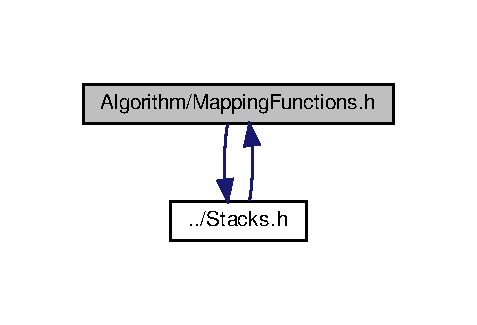
\includegraphics[width=229pt]{MappingFunctions_8h__incl}
\end{center}
\end{figure}
This graph shows which files directly or indirectly include this file\+:
\nopagebreak
\begin{figure}[H]
\begin{center}
\leavevmode
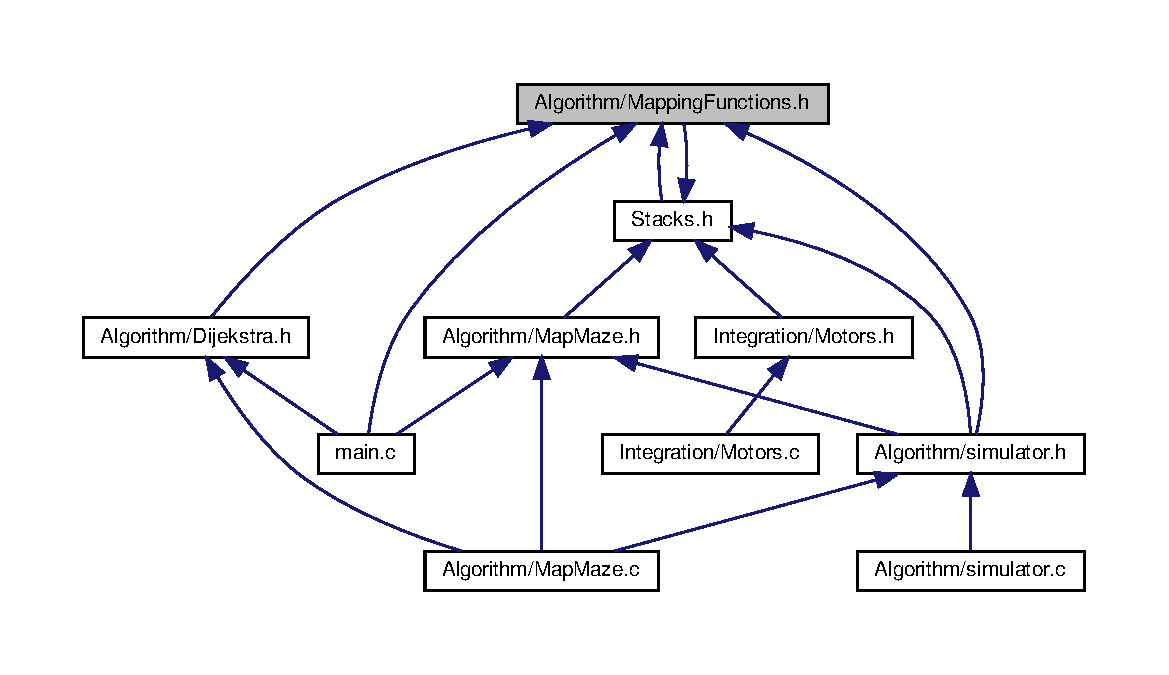
\includegraphics[width=350pt]{MappingFunctions_8h__dep__incl}
\end{center}
\end{figure}
\subsection*{Classes}
\begin{DoxyCompactItemize}
\item 
struct \hyperlink{structconnection}{connection}
\begin{DoxyCompactList}\small\item\em Connection between 2 nodes. \end{DoxyCompactList}\item 
struct \hyperlink{structNode}{Node}
\begin{DoxyCompactList}\small\item\em All info about a given \hyperlink{structNode}{Node}. \end{DoxyCompactList}\item 
struct \hyperlink{structcell}{cell}
\begin{DoxyCompactList}\small\item\em All info about a given cell. \end{DoxyCompactList}\item 
struct \hyperlink{structMaze}{Maze}
\begin{DoxyCompactList}\small\item\em Contains the representation of the maze itself. \end{DoxyCompactList}\end{DoxyCompactItemize}
\subsection*{Macros}
\begin{DoxyCompactItemize}
\item 
\#define \hyperlink{MappingFunctions_8h_abd2aacdca9cb2a1a30f3392256b96ea3}{M\+A\+X\+\_\+\+N\+O\+D\+ES}~22
\begin{DoxyCompactList}\small\item\em maximum number of Nodes that can be stored. \end{DoxyCompactList}\end{DoxyCompactItemize}
\begin{Indent}\textbf{ Maze Max Dimensions}\par
{\em The maximum dimensions the maze can be.

This section will determine the size of most of the arrays and so should be set to the smallest values that will definitely contain the entire maze. If it is set to small then the mouse will not explore the whole maze. }\begin{DoxyCompactItemize}
\item 
\#define \hyperlink{MappingFunctions_8h_a241aeeb764887ae5e3de58b98f04b16d}{W\+I\+D\+TH}~6
\item 
\#define \hyperlink{MappingFunctions_8h_aed89bd71aee8be823e8a20ec4e093c1e}{H\+E\+I\+G\+HT}~8
\item 
\#define \hyperlink{MappingFunctions_8h_a566d2490ad1a61a7a3079a6206c34bd9}{M\+A\+X\+\_\+\+D\+I\+M\+E\+N\+S\+I\+O\+NS}
\end{DoxyCompactItemize}
\end{Indent}
\textbf{ }\par
\begin{DoxyCompactItemize}
\item 
\mbox{\Hypertarget{MappingFunctions_8h_ab9a3c000d08d7bc3809090b0d91e6d15}\label{MappingFunctions_8h_ab9a3c000d08d7bc3809090b0d91e6d15}} 
\#define \hyperlink{MappingFunctions_8h_ab9a3c000d08d7bc3809090b0d91e6d15}{T\+U\+R\+N\+\_\+\+C\+O\+ST}~3
\begin{DoxyCompactList}\small\item\em cost of the movements between Nodes. \end{DoxyCompactList}\item 
\mbox{\Hypertarget{MappingFunctions_8h_ade770e395ba7136d47f13089d9ecfdf8}\label{MappingFunctions_8h_ade770e395ba7136d47f13089d9ecfdf8}} 
\#define {\bfseries S\+T\+R\+A\+I\+G\+H\+T\+\_\+\+C\+O\+ST}~1
\end{DoxyCompactItemize}

\subsection*{Typedefs}
\begin{DoxyCompactItemize}
\item 
\mbox{\Hypertarget{MappingFunctions_8h_a0466fc5f1bc9e6de776e48149b19c471}\label{MappingFunctions_8h_a0466fc5f1bc9e6de776e48149b19c471}} 
typedef struct \hyperlink{structNode}{Node} \hyperlink{MappingFunctions_8h_a0466fc5f1bc9e6de776e48149b19c471}{Node}
\begin{DoxyCompactList}\small\item\em All info about a given \hyperlink{structNode}{Node}. \end{DoxyCompactList}\item 
\mbox{\Hypertarget{MappingFunctions_8h_a7d3e730b07d2c8df607a2e561d1911ce}\label{MappingFunctions_8h_a7d3e730b07d2c8df607a2e561d1911ce}} 
typedef struct \hyperlink{structcell}{cell} \hyperlink{MappingFunctions_8h_a7d3e730b07d2c8df607a2e561d1911ce}{cell}
\begin{DoxyCompactList}\small\item\em All info about a given cell. \end{DoxyCompactList}\end{DoxyCompactItemize}
\subsection*{Functions}
\begin{DoxyCompactItemize}
\item 
unsigned char \hyperlink{MappingFunctions_8h_ab1cb7abf977587694dab1ef4c39de52f}{turn} (unsigned char N, unsigned char dir)
\begin{DoxyCompactList}\small\item\em Turn the right mouse within the virtual maze. \end{DoxyCompactList}\item 
unsigned char \hyperlink{MappingFunctions_8h_ac9d82259600ca30aa33430d3ae345533}{increment\+Index} (unsigned char index, unsigned char dir)
\begin{DoxyCompactList}\small\item\em Changes the index of the mouse to move into an adjacent cell. \end{DoxyCompactList}\end{DoxyCompactItemize}


\subsection{Detailed Description}
contains all functions, structures and data types used by most files. 

Functions are used throughout the program, mostly to edit the maze information. Structures that are used to store info about the maze are defined in this header so can be accessed from any file that includes it. This will be necessary for almost all navigating of the maze.

\begin{DoxyAuthor}{Author}
Nick Appleton @ U\+WE Robotics
\end{DoxyAuthor}
\begin{DoxyDate}{Date}
21/2/19 
\end{DoxyDate}


\subsection{Macro Definition Documentation}
\mbox{\Hypertarget{MappingFunctions_8h_aed89bd71aee8be823e8a20ec4e093c1e}\label{MappingFunctions_8h_aed89bd71aee8be823e8a20ec4e093c1e}} 
\index{Mapping\+Functions.\+h@{Mapping\+Functions.\+h}!H\+E\+I\+G\+HT@{H\+E\+I\+G\+HT}}
\index{H\+E\+I\+G\+HT@{H\+E\+I\+G\+HT}!Mapping\+Functions.\+h@{Mapping\+Functions.\+h}}
\subsubsection{\texorpdfstring{H\+E\+I\+G\+HT}{HEIGHT}}
{\footnotesize\ttfamily \#define H\+E\+I\+G\+HT~8}

height of the maze to be solved. If maze height is not known, set as largest value maze width that could occour. \mbox{\Hypertarget{MappingFunctions_8h_a566d2490ad1a61a7a3079a6206c34bd9}\label{MappingFunctions_8h_a566d2490ad1a61a7a3079a6206c34bd9}} 
\index{Mapping\+Functions.\+h@{Mapping\+Functions.\+h}!M\+A\+X\+\_\+\+D\+I\+M\+E\+N\+S\+I\+O\+NS@{M\+A\+X\+\_\+\+D\+I\+M\+E\+N\+S\+I\+O\+NS}}
\index{M\+A\+X\+\_\+\+D\+I\+M\+E\+N\+S\+I\+O\+NS@{M\+A\+X\+\_\+\+D\+I\+M\+E\+N\+S\+I\+O\+NS}!Mapping\+Functions.\+h@{Mapping\+Functions.\+h}}
\subsubsection{\texorpdfstring{M\+A\+X\+\_\+\+D\+I\+M\+E\+N\+S\+I\+O\+NS}{MAX\_DIMENSIONS}}
{\footnotesize\ttfamily \#define M\+A\+X\+\_\+\+D\+I\+M\+E\+N\+S\+I\+O\+NS}

marker to check if dimensions already defined. \mbox{\Hypertarget{MappingFunctions_8h_abd2aacdca9cb2a1a30f3392256b96ea3}\label{MappingFunctions_8h_abd2aacdca9cb2a1a30f3392256b96ea3}} 
\index{Mapping\+Functions.\+h@{Mapping\+Functions.\+h}!M\+A\+X\+\_\+\+N\+O\+D\+ES@{M\+A\+X\+\_\+\+N\+O\+D\+ES}}
\index{M\+A\+X\+\_\+\+N\+O\+D\+ES@{M\+A\+X\+\_\+\+N\+O\+D\+ES}!Mapping\+Functions.\+h@{Mapping\+Functions.\+h}}
\subsubsection{\texorpdfstring{M\+A\+X\+\_\+\+N\+O\+D\+ES}{MAX\_NODES}}
{\footnotesize\ttfamily \#define M\+A\+X\+\_\+\+N\+O\+D\+ES~22}



maximum number of Nodes that can be stored. 

describes the amount of memory needed to store the list of Nodes. Will not be able to store more Nodes than this. \mbox{\Hypertarget{MappingFunctions_8h_a241aeeb764887ae5e3de58b98f04b16d}\label{MappingFunctions_8h_a241aeeb764887ae5e3de58b98f04b16d}} 
\index{Mapping\+Functions.\+h@{Mapping\+Functions.\+h}!W\+I\+D\+TH@{W\+I\+D\+TH}}
\index{W\+I\+D\+TH@{W\+I\+D\+TH}!Mapping\+Functions.\+h@{Mapping\+Functions.\+h}}
\subsubsection{\texorpdfstring{W\+I\+D\+TH}{WIDTH}}
{\footnotesize\ttfamily \#define W\+I\+D\+TH~6}

Width of the maze to be solved. If maze width is not known, set as largest value maze width that could occour. 

\subsection{Function Documentation}
\mbox{\Hypertarget{MappingFunctions_8h_ac9d82259600ca30aa33430d3ae345533}\label{MappingFunctions_8h_ac9d82259600ca30aa33430d3ae345533}} 
\index{Mapping\+Functions.\+h@{Mapping\+Functions.\+h}!increment\+Index@{increment\+Index}}
\index{increment\+Index@{increment\+Index}!Mapping\+Functions.\+h@{Mapping\+Functions.\+h}}
\subsubsection{\texorpdfstring{increment\+Index()}{incrementIndex()}}
{\footnotesize\ttfamily unsigned char increment\+Index (\begin{DoxyParamCaption}\item[{unsigned char}]{index,  }\item[{unsigned char}]{dir }\end{DoxyParamCaption})}



Changes the index of the mouse to move into an adjacent cell. 

looks at the direction the mouse is facing and changes the index by the right amount to move the mouse into the adjacent cell in that direction.


\begin{DoxyParams}{Parameters}
{\em index} & index to be incremented. \\
\hline
{\em dir} & direction to move into. \\
\hline
\end{DoxyParams}
\begin{DoxyReturn}{Returns}
the index having been incremented into the adjacent cell. 
\end{DoxyReturn}
\mbox{\Hypertarget{MappingFunctions_8h_ab1cb7abf977587694dab1ef4c39de52f}\label{MappingFunctions_8h_ab1cb7abf977587694dab1ef4c39de52f}} 
\index{Mapping\+Functions.\+h@{Mapping\+Functions.\+h}!turn@{turn}}
\index{turn@{turn}!Mapping\+Functions.\+h@{Mapping\+Functions.\+h}}
\subsubsection{\texorpdfstring{turn()}{turn()}}
{\footnotesize\ttfamily unsigned char turn (\begin{DoxyParamCaption}\item[{unsigned char}]{N,  }\item[{unsigned char}]{dir }\end{DoxyParamCaption})}



Turn the right mouse within the virtual maze. 

Bitshifts the direction register of the mouse right by N places. Also corrects for if the 1 bit falls off the end of the register.


\begin{DoxyParams}{Parameters}
{\em N} & Number of turns to make. \\
\hline
{\em dir} & Current direction to be turned. \\
\hline
\end{DoxyParams}
\begin{DoxyReturn}{Returns}
New direction after turning 
\end{DoxyReturn}

\hypertarget{simulator_8c}{}\section{Algorithm/simulator.c File Reference}
\label{simulator_8c}\index{Algorithm/simulator.\+c@{Algorithm/simulator.\+c}}


Display the maze for debugging.  


{\ttfamily \#include \char`\"{}simulator.\+h\char`\"{}}\newline
{\ttfamily \#include $<$stdio.\+h$>$}\newline
Include dependency graph for simulator.\+c\+:
\nopagebreak
\begin{figure}[H]
\begin{center}
\leavevmode
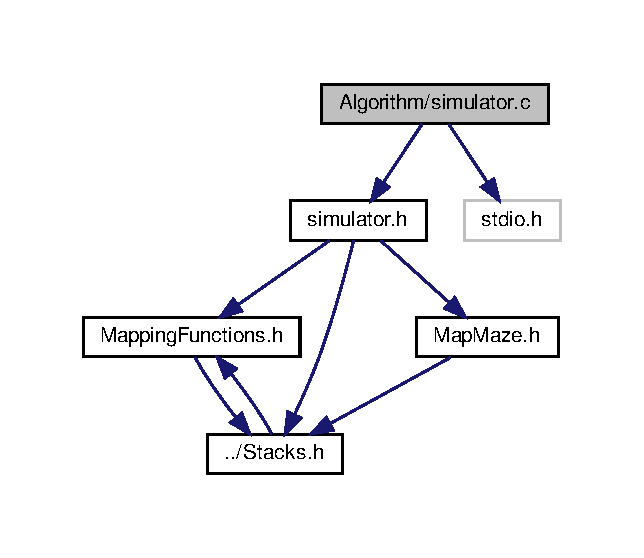
\includegraphics[width=309pt]{simulator_8c__incl}
\end{center}
\end{figure}
\subsection*{Macros}
\begin{Indent}\textbf{ Maze Actual Simulated Dimensions}\par
{\em The actual size of the simulated maze.

This section defines sizes that the simulated maze actually is. The maze is used in the read\+Sensors function as all the other functions will refer to the mouses view of the maze. }\begin{DoxyCompactItemize}
\item 
\#define \hyperlink{simulator_8c_abf766f80723946ab81de447490748744}{A\+C\+T\+U\+A\+L\+\_\+\+W\+I\+D\+TH}~6
\item 
\#define \hyperlink{simulator_8c_ad6967ee13d58faee6aec23fb7e6494da}{A\+C\+T\+U\+A\+L\+\_\+\+H\+E\+I\+G\+HT}~8
\end{DoxyCompactItemize}
\end{Indent}
\subsection*{Functions}
\begin{DoxyCompactItemize}
\item 
int \hyperlink{simulator_8c_aa5ab68e883f48468965e2864b55f4759}{Wall\+\_\+\+Check} (unsigned char index, unsigned char direction)
\begin{DoxyCompactList}\small\item\em used to find if a wall is there or not. \end{DoxyCompactList}\item 
void \hyperlink{simulator_8c_ac6e138e1843b45c00214e66b975b912e}{print\+Status} (\hyperlink{structMouse}{Mouse} $\ast$\hyperlink{MapMaze_8c_a07faa847230d0abd8c3db00e3f8cae7a}{mouse}, \hyperlink{structStack}{Stack} $\ast$openlist, \hyperlink{structNode}{Node} $\ast$nodelist)
\begin{DoxyCompactList}\small\item\em Print out the maze to stdout. \end{DoxyCompactList}\item 
void \hyperlink{simulator_8c_a3f607ad9cc68bfb0c710be0893a867e0}{Turn} (int direciton)
\begin{DoxyCompactList}\small\item\em Turn physical \hyperlink{structMouse}{Mouse}. \end{DoxyCompactList}\item 
void \hyperlink{simulator_8c_a324b4be9e04c414eda8564c949fed51f}{Fwd\+\_\+\+One\+\_\+\+Cell} (void)
\begin{DoxyCompactList}\small\item\em Move physical mouse forward one cell. \end{DoxyCompactList}\item 
\mbox{\Hypertarget{simulator_8c_ad9b144f0c677a8f7b2434f4d8b441756}\label{simulator_8c_ad9b144f0c677a8f7b2434f4d8b441756}} 
void {\bfseries Fast\+\_\+\+Run} (\hyperlink{structStack}{Stack} route, int \hyperlink{IO_8c_a481cb487704fc7f8c8ddc6613aed3785}{speed})
\item 
\mbox{\Hypertarget{simulator_8c_abaf2ecf718b0d21a6aa28e54c1951c54}\label{simulator_8c_abaf2ecf718b0d21a6aa28e54c1951c54}} 
void {\bfseries Fast\+Turn} (int dir)
\end{DoxyCompactItemize}


\subsection{Detailed Description}
Display the maze for debugging. 

Adds functionality for the simulator to be used. This will mean that the program can be run without using the physical Micromouse. The functions have the same name as in the non-\/ simulator functions so by defining S\+I\+M\+U\+L\+A\+T\+OR in the main it will run these instead of the actual mouse integratiion funtions.

\begin{DoxyAuthor}{Author}
Nick Appleton @ U\+WE Robotics
\end{DoxyAuthor}
\begin{DoxyDate}{Date}
22/2/19 
\end{DoxyDate}


\subsection{Macro Definition Documentation}
\mbox{\Hypertarget{simulator_8c_ad6967ee13d58faee6aec23fb7e6494da}\label{simulator_8c_ad6967ee13d58faee6aec23fb7e6494da}} 
\index{simulator.\+c@{simulator.\+c}!A\+C\+T\+U\+A\+L\+\_\+\+H\+E\+I\+G\+HT@{A\+C\+T\+U\+A\+L\+\_\+\+H\+E\+I\+G\+HT}}
\index{A\+C\+T\+U\+A\+L\+\_\+\+H\+E\+I\+G\+HT@{A\+C\+T\+U\+A\+L\+\_\+\+H\+E\+I\+G\+HT}!simulator.\+c@{simulator.\+c}}
\subsubsection{\texorpdfstring{A\+C\+T\+U\+A\+L\+\_\+\+H\+E\+I\+G\+HT}{ACTUAL\_HEIGHT}}
{\footnotesize\ttfamily \#define A\+C\+T\+U\+A\+L\+\_\+\+H\+E\+I\+G\+HT~8}

the Height the simulated maze actually is \mbox{\Hypertarget{simulator_8c_abf766f80723946ab81de447490748744}\label{simulator_8c_abf766f80723946ab81de447490748744}} 
\index{simulator.\+c@{simulator.\+c}!A\+C\+T\+U\+A\+L\+\_\+\+W\+I\+D\+TH@{A\+C\+T\+U\+A\+L\+\_\+\+W\+I\+D\+TH}}
\index{A\+C\+T\+U\+A\+L\+\_\+\+W\+I\+D\+TH@{A\+C\+T\+U\+A\+L\+\_\+\+W\+I\+D\+TH}!simulator.\+c@{simulator.\+c}}
\subsubsection{\texorpdfstring{A\+C\+T\+U\+A\+L\+\_\+\+W\+I\+D\+TH}{ACTUAL\_WIDTH}}
{\footnotesize\ttfamily \#define A\+C\+T\+U\+A\+L\+\_\+\+W\+I\+D\+TH~6}

the Width the simulated maze actually is 

\subsection{Function Documentation}
\mbox{\Hypertarget{simulator_8c_a324b4be9e04c414eda8564c949fed51f}\label{simulator_8c_a324b4be9e04c414eda8564c949fed51f}} 
\index{simulator.\+c@{simulator.\+c}!Fwd\+\_\+\+One\+\_\+\+Cell@{Fwd\+\_\+\+One\+\_\+\+Cell}}
\index{Fwd\+\_\+\+One\+\_\+\+Cell@{Fwd\+\_\+\+One\+\_\+\+Cell}!simulator.\+c@{simulator.\+c}}
\subsubsection{\texorpdfstring{Fwd\+\_\+\+One\+\_\+\+Cell()}{Fwd\_One\_Cell()}}
{\footnotesize\ttfamily void Fwd\+\_\+\+One\+\_\+\+Cell (\begin{DoxyParamCaption}\item[{void}]{ }\end{DoxyParamCaption})}



Move physical mouse forward one cell. 

move the mouse forward one cell.

Dummy function as there is no physical mouse to turn. This is a placeholder so that the final program will run correctly on the simulator with minimal changing of code. \mbox{\Hypertarget{simulator_8c_ac6e138e1843b45c00214e66b975b912e}\label{simulator_8c_ac6e138e1843b45c00214e66b975b912e}} 
\index{simulator.\+c@{simulator.\+c}!print\+Status@{print\+Status}}
\index{print\+Status@{print\+Status}!simulator.\+c@{simulator.\+c}}
\subsubsection{\texorpdfstring{print\+Status()}{printStatus()}}
{\footnotesize\ttfamily void print\+Status (\begin{DoxyParamCaption}\item[{\hyperlink{structMouse}{Mouse} $\ast$}]{mouse,  }\item[{\hyperlink{structStack}{Stack} $\ast$}]{openlist,  }\item[{\hyperlink{structNode}{Node} $\ast$}]{nodelist }\end{DoxyParamCaption})}



Print out the maze to stdout. 

Prints the maze in it\textquotesingle{}s current state to the standard output, including state of the L\+E\+Ds, position and direction of the mouse and the mouse\textquotesingle{}s model of the maze -\/ this will display the walls and nodes graphically.


\begin{DoxyParams}{Parameters}
{\em mouse} & representation of the mouse to be referenced. \\
\hline
\end{DoxyParams}
\mbox{\Hypertarget{simulator_8c_a3f607ad9cc68bfb0c710be0893a867e0}\label{simulator_8c_a3f607ad9cc68bfb0c710be0893a867e0}} 
\index{simulator.\+c@{simulator.\+c}!Turn@{Turn}}
\index{Turn@{Turn}!simulator.\+c@{simulator.\+c}}
\subsubsection{\texorpdfstring{Turn()}{Turn()}}
{\footnotesize\ttfamily void Turn (\begin{DoxyParamCaption}\item[{int}]{direciton }\end{DoxyParamCaption})}



Turn physical \hyperlink{structMouse}{Mouse}. 

turn the mouse 90 degrees in a given direction.

Dummy function as there is no physical mouse to turn. This is a placeholder so that the final program will run correctly on the simulator with minimal changing of code.


\begin{DoxyParams}{Parameters}
{\em direciton} & Direction to turn. \\
\hline
\end{DoxyParams}
\mbox{\Hypertarget{simulator_8c_aa5ab68e883f48468965e2864b55f4759}\label{simulator_8c_aa5ab68e883f48468965e2864b55f4759}} 
\index{simulator.\+c@{simulator.\+c}!Wall\+\_\+\+Check@{Wall\+\_\+\+Check}}
\index{Wall\+\_\+\+Check@{Wall\+\_\+\+Check}!simulator.\+c@{simulator.\+c}}
\subsubsection{\texorpdfstring{Wall\+\_\+\+Check()}{Wall\_Check()}}
{\footnotesize\ttfamily int Wall\+\_\+\+Check (\begin{DoxyParamCaption}\item[{unsigned char}]{index,  }\item[{unsigned char}]{direction }\end{DoxyParamCaption})}



used to find if a wall is there or not. 

contains the array of the actual maze walls and uses the index and direction of the mouse to determine if there is a wall or not. This is a simulated version of reading the sensor values and passing a 1 or 0 depending on the status of the wall.


\begin{DoxyParams}{Parameters}
{\em index} & index that the mouse is at within the maze. \\
\hline
{\em direction} & direction register of the mouse. \\
\hline
\end{DoxyParams}
Which wall is being checked 
\hypertarget{IO_8c}{}\section{Integration/\+IO.c File Reference}
\label{IO_8c}\index{Integration/\+I\+O.\+c@{Integration/\+I\+O.\+c}}


Functions for input and output Integration.  


{\ttfamily \#include \char`\"{}Setup.\+h\char`\"{}}\newline
{\ttfamily \#include \char`\"{}I\+O.\+h\char`\"{}}\newline
{\ttfamily \#include $<$p30\+Fxxxx.\+h$>$}\newline
Include dependency graph for I\+O.\+c\+:
\nopagebreak
\begin{figure}[H]
\begin{center}
\leavevmode
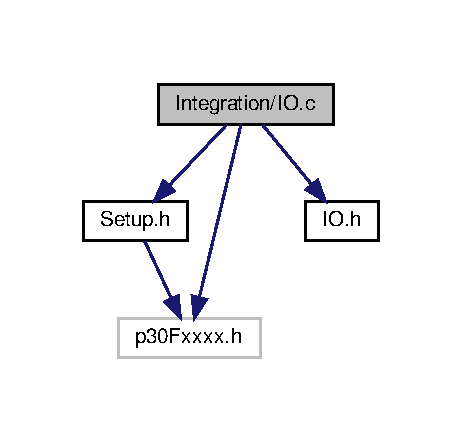
\includegraphics[width=222pt]{IO_8c__incl}
\end{center}
\end{figure}
\subsection*{Macros}
\begin{DoxyCompactItemize}
\item 
\#define \hyperlink{IO_8c_ae70d49989e387fc76c7e21607f094778}{no\+Wall}~10
\end{DoxyCompactItemize}
\textbf{ }\par
\begin{DoxyCompactItemize}
\item 
\mbox{\Hypertarget{IO_8c_a99ad70af8ff9fce7b7141201a3ee2dc6}\label{IO_8c_a99ad70af8ff9fce7b7141201a3ee2dc6}} 
\#define \hyperlink{IO_8c_a99ad70af8ff9fce7b7141201a3ee2dc6}{upper\+Error}~10
\begin{DoxyCompactList}\small\item\em thresholds for anomilous sensor values used in P\+ID \end{DoxyCompactList}\item 
\mbox{\Hypertarget{IO_8c_acf6b905fc6a9f8b8bd4c13199f746be7}\label{IO_8c_acf6b905fc6a9f8b8bd4c13199f746be7}} 
\#define {\bfseries lower\+Error}~10
\end{DoxyCompactItemize}

\subsection*{Functions}
\begin{DoxyCompactItemize}
\item 
void \hyperlink{IO_8c_a226557d5e42f7e29ddaff30606138459}{\+\_\+\+\_\+attribute\+\_\+\+\_\+} ((interrupt, no\+\_\+auto\+\_\+psv))
\begin{DoxyCompactList}\small\item\em U\+A\+RT 2 receive interrupt for encoder 2 and U\+SB interface. \end{DoxyCompactList}\item 
float \hyperlink{IO_8c_a5ce20c906e202258abde90ad5ac5f975}{Sensor\+\_\+\+Read} (int sensor)
\begin{DoxyCompactList}\small\item\em read the Sensors using the A\+DC. \end{DoxyCompactList}\item 
void \hyperlink{IO_8c_a4dda47d5c64a5471c6321138c570dcc5}{Start\+\_\+\+Position} (void)
\begin{DoxyCompactList}\small\item\em Use L\+E\+Ds to give feedback on position in cell. \end{DoxyCompactList}\item 
void \hyperlink{IO_8c_a30b6155e77b7ff2de2da47c456769428}{Sensor\+\_\+\+Test} (void)
\begin{DoxyCompactList}\small\item\em check if there is a wall or not. \end{DoxyCompactList}\item 
void \hyperlink{IO_8c_a348b663f86a656f5ea991d496ff9b896}{\+\_\+\+\_\+attribute\+\_\+\+\_\+} ((interrupt, auto\+\_\+psv))
\begin{DoxyCompactList}\small\item\em Timer1 interrupt for L\+ED display. \end{DoxyCompactList}\item 
void \hyperlink{IO_8c_a4d8df502b7da76dda97312ec92b30ecf}{Set\+L\+ED} (unsigned char L\+ED, unsigned char set)
\begin{DoxyCompactList}\small\item\em Turn L\+ED on or off. \end{DoxyCompactList}\item 
void \hyperlink{IO_8c_a6cdc25769fbef821b96dd6c995e9479c}{Display} (unsigned char setmode, unsigned int speedchange)
\begin{DoxyCompactList}\small\item\em Set what is displayed on the L\+E\+Ds. \end{DoxyCompactList}\end{DoxyCompactItemize}
\subsection*{Variables}
\begin{DoxyCompactItemize}
\item 
\mbox{\Hypertarget{IO_8c_aa359a6a5a50c709ba1c7ba1668c2b518}\label{IO_8c_aa359a6a5a50c709ba1c7ba1668c2b518}} 
unsigned char \hyperlink{IO_8c_aa359a6a5a50c709ba1c7ba1668c2b518}{sensor\+Val}
\begin{DoxyCompactList}\small\item\em Value read by the sensor. Global because it is used in the interrupt. \end{DoxyCompactList}\item 
unsigned int \hyperlink{IO_8c_a481cb487704fc7f8c8ddc6613aed3785}{speed}
\item 
unsigned char \hyperlink{IO_8c_a74b654271a172a244c844fb86277cd8a}{mode}
\end{DoxyCompactItemize}


\subsection{Detailed Description}
Functions for input and output Integration. 

Includes the interrupts for sensor inputs and L\+ED outputs as well as functions to decode values and make use of the IO

\begin{DoxyAuthor}{Author}
Christian Woof @ U\+WE Robotics 
\end{DoxyAuthor}


\subsection{Macro Definition Documentation}
\mbox{\Hypertarget{IO_8c_ae70d49989e387fc76c7e21607f094778}\label{IO_8c_ae70d49989e387fc76c7e21607f094778}} 
\index{I\+O.\+c@{I\+O.\+c}!no\+Wall@{no\+Wall}}
\index{no\+Wall@{no\+Wall}!I\+O.\+c@{I\+O.\+c}}
\subsubsection{\texorpdfstring{no\+Wall}{noWall}}
{\footnotesize\ttfamily \#define no\+Wall~10}

threshold for if a wall has been sensed. 

\subsection{Function Documentation}
\mbox{\Hypertarget{IO_8c_a226557d5e42f7e29ddaff30606138459}\label{IO_8c_a226557d5e42f7e29ddaff30606138459}} 
\index{I\+O.\+c@{I\+O.\+c}!\+\_\+\+\_\+attribute\+\_\+\+\_\+@{\+\_\+\+\_\+attribute\+\_\+\+\_\+}}
\index{\+\_\+\+\_\+attribute\+\_\+\+\_\+@{\+\_\+\+\_\+attribute\+\_\+\+\_\+}!I\+O.\+c@{I\+O.\+c}}
\subsubsection{\texorpdfstring{\+\_\+\+\_\+attribute\+\_\+\+\_\+()}{\_\_attribute\_\_()}\hspace{0.1cm}{\footnotesize\ttfamily [1/2]}}
{\footnotesize\ttfamily void \+\_\+\+\_\+attribute\+\_\+\+\_\+ (\begin{DoxyParamCaption}\item[{(interrupt, no\+\_\+auto\+\_\+psv)}]{ }\end{DoxyParamCaption})}



U\+A\+RT 2 receive interrupt for encoder 2 and U\+SB interface. 

U\+A\+RT 1 receive interrupt for encoder 1 and programmer.

A\+DC interrupt for use with sensors. \mbox{\Hypertarget{IO_8c_a348b663f86a656f5ea991d496ff9b896}\label{IO_8c_a348b663f86a656f5ea991d496ff9b896}} 
\index{I\+O.\+c@{I\+O.\+c}!\+\_\+\+\_\+attribute\+\_\+\+\_\+@{\+\_\+\+\_\+attribute\+\_\+\+\_\+}}
\index{\+\_\+\+\_\+attribute\+\_\+\+\_\+@{\+\_\+\+\_\+attribute\+\_\+\+\_\+}!I\+O.\+c@{I\+O.\+c}}
\subsubsection{\texorpdfstring{\+\_\+\+\_\+attribute\+\_\+\+\_\+()}{\_\_attribute\_\_()}\hspace{0.1cm}{\footnotesize\ttfamily [2/2]}}
{\footnotesize\ttfamily void \+\_\+\+\_\+attribute\+\_\+\+\_\+ (\begin{DoxyParamCaption}\item[{(interrupt, auto\+\_\+psv)}]{ }\end{DoxyParamCaption})}



Timer1 interrupt for L\+ED display. 

reset the timer 1 interrupt flag \mbox{\Hypertarget{IO_8c_a6cdc25769fbef821b96dd6c995e9479c}\label{IO_8c_a6cdc25769fbef821b96dd6c995e9479c}} 
\index{I\+O.\+c@{I\+O.\+c}!Display@{Display}}
\index{Display@{Display}!I\+O.\+c@{I\+O.\+c}}
\subsubsection{\texorpdfstring{Display()}{Display()}}
{\footnotesize\ttfamily void Display (\begin{DoxyParamCaption}\item[{unsigned char}]{setmode,  }\item[{unsigned int}]{speedchange }\end{DoxyParamCaption})}



Set what is displayed on the L\+E\+Ds. 


\begin{DoxyParams}{Parameters}
{\em setmode} & Which display Mode is to be used. \\
\hline
{\em speedchange} & Speed the display should go at. \\
\hline
\end{DoxyParams}
\mbox{\Hypertarget{IO_8c_a5ce20c906e202258abde90ad5ac5f975}\label{IO_8c_a5ce20c906e202258abde90ad5ac5f975}} 
\index{I\+O.\+c@{I\+O.\+c}!Sensor\+\_\+\+Read@{Sensor\+\_\+\+Read}}
\index{Sensor\+\_\+\+Read@{Sensor\+\_\+\+Read}!I\+O.\+c@{I\+O.\+c}}
\subsubsection{\texorpdfstring{Sensor\+\_\+\+Read()}{Sensor\_Read()}}
{\footnotesize\ttfamily float Sensor\+\_\+\+Read (\begin{DoxyParamCaption}\item[{int}]{sensor }\end{DoxyParamCaption})}



read the Sensors using the A\+DC. 


\begin{DoxyParams}{Parameters}
{\em sensor} & which sensor to read from. \\
\hline
\end{DoxyParams}
\begin{DoxyReturn}{Returns}
value between 0 and 255 of sensor read. 
\end{DoxyReturn}
\mbox{\Hypertarget{IO_8c_a30b6155e77b7ff2de2da47c456769428}\label{IO_8c_a30b6155e77b7ff2de2da47c456769428}} 
\index{I\+O.\+c@{I\+O.\+c}!Sensor\+\_\+\+Test@{Sensor\+\_\+\+Test}}
\index{Sensor\+\_\+\+Test@{Sensor\+\_\+\+Test}!I\+O.\+c@{I\+O.\+c}}
\subsubsection{\texorpdfstring{Sensor\+\_\+\+Test()}{Sensor\_Test()}}
{\footnotesize\ttfamily void Sensor\+\_\+\+Test (\begin{DoxyParamCaption}\item[{void}]{ }\end{DoxyParamCaption})}



check if there is a wall or not. 

Uses \hyperlink{IO_8c_a5ce20c906e202258abde90ad5ac5f975}{Sensor\+\_\+\+Read()} to get an average of the sensor values and uses this to determine whether there is a wall or not in the direciton of the sensor.


\begin{DoxyParams}{Parameters}
{\em side} & which side of the mouse is being checked. \\
\hline
\end{DoxyParams}
\begin{DoxyReturn}{Returns}
1 or 0 (Wall or no Wall). Test sensors 
\end{DoxyReturn}
\mbox{\Hypertarget{IO_8c_a4d8df502b7da76dda97312ec92b30ecf}\label{IO_8c_a4d8df502b7da76dda97312ec92b30ecf}} 
\index{I\+O.\+c@{I\+O.\+c}!Set\+L\+ED@{Set\+L\+ED}}
\index{Set\+L\+ED@{Set\+L\+ED}!I\+O.\+c@{I\+O.\+c}}
\subsubsection{\texorpdfstring{Set\+L\+E\+D()}{SetLED()}}
{\footnotesize\ttfamily void Set\+L\+ED (\begin{DoxyParamCaption}\item[{unsigned char}]{L\+ED,  }\item[{unsigned char}]{set }\end{DoxyParamCaption})}



Turn L\+ED on or off. 


\begin{DoxyParams}{Parameters}
{\em L\+ED} & which L\+ED is being set. \\
\hline
{\em set} & Set or Clear. \\
\hline
\end{DoxyParams}
\mbox{\Hypertarget{IO_8c_a4dda47d5c64a5471c6321138c570dcc5}\label{IO_8c_a4dda47d5c64a5471c6321138c570dcc5}} 
\index{I\+O.\+c@{I\+O.\+c}!Start\+\_\+\+Position@{Start\+\_\+\+Position}}
\index{Start\+\_\+\+Position@{Start\+\_\+\+Position}!I\+O.\+c@{I\+O.\+c}}
\subsubsection{\texorpdfstring{Start\+\_\+\+Position()}{Start\_Position()}}
{\footnotesize\ttfamily void Start\+\_\+\+Position (\begin{DoxyParamCaption}\item[{void}]{ }\end{DoxyParamCaption})}



Use L\+E\+Ds to give feedback on position in cell. 

used to setup the mouse in the maze at the beginning by holding the mouse in the cell until the 2 L\+E\+Ds turn off. This means that the mouse is in the correct position. 

\subsection{Variable Documentation}
\mbox{\Hypertarget{IO_8c_a74b654271a172a244c844fb86277cd8a}\label{IO_8c_a74b654271a172a244c844fb86277cd8a}} 
\index{I\+O.\+c@{I\+O.\+c}!mode@{mode}}
\index{mode@{mode}!I\+O.\+c@{I\+O.\+c}}
\subsubsection{\texorpdfstring{mode}{mode}}
{\footnotesize\ttfamily unsigned char mode}

L\+ED mode to be displayed \mbox{\Hypertarget{IO_8c_a481cb487704fc7f8c8ddc6613aed3785}\label{IO_8c_a481cb487704fc7f8c8ddc6613aed3785}} 
\index{I\+O.\+c@{I\+O.\+c}!speed@{speed}}
\index{speed@{speed}!I\+O.\+c@{I\+O.\+c}}
\subsubsection{\texorpdfstring{speed}{speed}}
{\footnotesize\ttfamily unsigned int speed}

speed at which the L\+ED patterns will be displayed. 
\hypertarget{Motors_8c}{}\section{Integration/\+Motors.c File Reference}
\label{Motors_8c}\index{Integration/\+Motors.\+c@{Integration/\+Motors.\+c}}


Motor Functions and Defines.  


{\ttfamily \#include \char`\"{}Setup.\+h\char`\"{}}\newline
{\ttfamily \#include \char`\"{}I\+O.\+h\char`\"{}}\newline
{\ttfamily \#include \char`\"{}Motors.\+h\char`\"{}}\newline
Include dependency graph for Motors.\+c\+:
\nopagebreak
\begin{figure}[H]
\begin{center}
\leavevmode
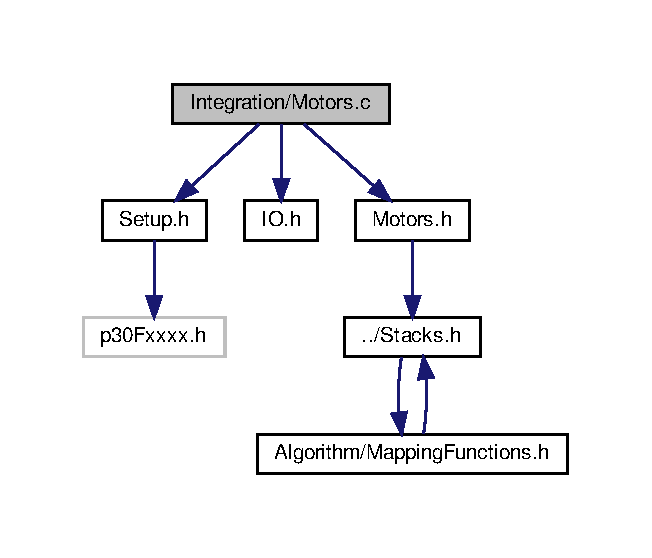
\includegraphics[width=313pt]{Motors_8c__incl}
\end{center}
\end{figure}
\subsection*{Functions}
\begin{DoxyCompactItemize}
\item 
float \hyperlink{Motors_8c_a9a09ab1256a3fb60fec7a786de4fbfdc}{P\+ID} (int close\+\_\+\+Sensor\+\_\+\+Side)
\begin{DoxyCompactList}\small\item\em P\+ID controller for moving through the maze. \end{DoxyCompactList}\item 
void \hyperlink{Motors_8c_a226557d5e42f7e29ddaff30606138459}{\+\_\+\+\_\+attribute\+\_\+\+\_\+} ((interrupt, no\+\_\+auto\+\_\+psv))
\begin{DoxyCompactList}\small\item\em A\+DC interrupt for use with sensors. \end{DoxyCompactList}\item 
void \hyperlink{Motors_8c_a6d8a633e18359b5375fe00cdc74964ff}{Velocity\+\_\+\+Curve} (unsigned char direction)
\begin{DoxyCompactList}\small\item\em accelerate the mouse up to speed, or from speed to static. \end{DoxyCompactList}\item 
void \hyperlink{Motors_8c_a550c2e802fb3ecc724fc377a38312899}{Turn\+\_\+\+Velocity\+\_\+\+Curve} (unsigned char direction)
\begin{DoxyCompactList}\small\item\em accelerate or decelerate the mouse for the turns when exploring. \end{DoxyCompactList}\item 
void \hyperlink{Motors_8c_aa1f8e804eab7ce71bff408b7d89c52d6}{M\+\_\+\+Dir} (int M\+L\+Dir, int M\+R\+Dir)
\begin{DoxyCompactList}\small\item\em sets motor directions. \end{DoxyCompactList}\item 
void \hyperlink{Motors_8c_add90bf710ddc10212c0d3abec982a1d1}{Turn} (int \hyperlink{MappingFunctions_8h_ab1cb7abf977587694dab1ef4c39de52f}{turn})
\begin{DoxyCompactList}\small\item\em Turn physical \hyperlink{structMouse}{Mouse}. \end{DoxyCompactList}\item 
void \hyperlink{Motors_8c_a324b4be9e04c414eda8564c949fed51f}{Fwd\+\_\+\+One\+\_\+\+Cell} (void)
\begin{DoxyCompactList}\small\item\em Move physical mouse forward one cell. \end{DoxyCompactList}\item 
void \hyperlink{Motors_8c_a723968c7dd5070f3dab8cdcc72c45355}{Fast\+\_\+\+Run} (\hyperlink{structStack}{Stack} instructions, unsigned char \hyperlink{IO_8c_a481cb487704fc7f8c8ddc6613aed3785}{speed})
\begin{DoxyCompactList}\small\item\em complete a fast run of a stack of instructions. \end{DoxyCompactList}\item 
void \hyperlink{Motors_8c_ab2fa04584bc59ca4993e325c87aad36a}{Fwd} (int cells)
\begin{DoxyCompactList}\small\item\em move the mouse forward the number of cells given. \end{DoxyCompactList}\item 
void \hyperlink{Motors_8c_a27d46a52f8d8f190abe85888d35a5cf4}{Fast\+\_\+\+Turn} (unsigned char dir)
\begin{DoxyCompactList}\small\item\em make a turn at full speed. \end{DoxyCompactList}\end{DoxyCompactItemize}
\subsection*{Variables}
\textbf{ }\par
\begin{DoxyCompactItemize}
\item 
\mbox{\Hypertarget{Motors_8c_a09508bf842d31874b9cd2c1271d4b8de}\label{Motors_8c_a09508bf842d31874b9cd2c1271d4b8de}} 
int \hyperlink{Motors_8c_a09508bf842d31874b9cd2c1271d4b8de}{M\+L\+Enc\+Count}
\begin{DoxyCompactList}\small\item\em Encoder counts. \end{DoxyCompactList}\item 
\mbox{\Hypertarget{Motors_8c_acf3b0e8270d0e0cfc372fcce5ea98e0d}\label{Motors_8c_acf3b0e8270d0e0cfc372fcce5ea98e0d}} 
int {\bfseries M\+R\+Enc\+Count}
\end{DoxyCompactItemize}



\subsection{Detailed Description}
Motor Functions and Defines. 

\begin{DoxyAuthor}{Author}
Christian Woof @ U\+WE Robotics 
\end{DoxyAuthor}


\subsection{Function Documentation}
\mbox{\Hypertarget{Motors_8c_a226557d5e42f7e29ddaff30606138459}\label{Motors_8c_a226557d5e42f7e29ddaff30606138459}} 
\index{Motors.\+c@{Motors.\+c}!\+\_\+\+\_\+attribute\+\_\+\+\_\+@{\+\_\+\+\_\+attribute\+\_\+\+\_\+}}
\index{\+\_\+\+\_\+attribute\+\_\+\+\_\+@{\+\_\+\+\_\+attribute\+\_\+\+\_\+}!Motors.\+c@{Motors.\+c}}
\subsubsection{\texorpdfstring{\+\_\+\+\_\+attribute\+\_\+\+\_\+()}{\_\_attribute\_\_()}}
{\footnotesize\ttfamily void \+\_\+\+\_\+attribute\+\_\+\+\_\+ (\begin{DoxyParamCaption}\item[{(interrupt, no\+\_\+auto\+\_\+psv)}]{ }\end{DoxyParamCaption})}



A\+DC interrupt for use with sensors. 

U\+A\+RT 1 receive interrupt for encoder 1 and programmer.

A\+DC interrupt for use with sensors. \mbox{\Hypertarget{Motors_8c_a723968c7dd5070f3dab8cdcc72c45355}\label{Motors_8c_a723968c7dd5070f3dab8cdcc72c45355}} 
\index{Motors.\+c@{Motors.\+c}!Fast\+\_\+\+Run@{Fast\+\_\+\+Run}}
\index{Fast\+\_\+\+Run@{Fast\+\_\+\+Run}!Motors.\+c@{Motors.\+c}}
\subsubsection{\texorpdfstring{Fast\+\_\+\+Run()}{Fast\_Run()}}
{\footnotesize\ttfamily void Fast\+\_\+\+Run (\begin{DoxyParamCaption}\item[{\hyperlink{structStack}{Stack}}]{instructions,  }\item[{unsigned char}]{speed }\end{DoxyParamCaption})}



complete a fast run of a stack of instructions. 

follows the instructions in the given stack to get from the current location to the destination using the fast move functions. This will be used for the final run.


\begin{DoxyParams}{Parameters}
{\em instructions} & \hyperlink{structStack}{Stack} of instructions to follow to get to the destination. \\
\hline
{\em speed} & Whether it is going full or half speed. \\
\hline
\end{DoxyParams}
\mbox{\Hypertarget{Motors_8c_a27d46a52f8d8f190abe85888d35a5cf4}\label{Motors_8c_a27d46a52f8d8f190abe85888d35a5cf4}} 
\index{Motors.\+c@{Motors.\+c}!Fast\+\_\+\+Turn@{Fast\+\_\+\+Turn}}
\index{Fast\+\_\+\+Turn@{Fast\+\_\+\+Turn}!Motors.\+c@{Motors.\+c}}
\subsubsection{\texorpdfstring{Fast\+\_\+\+Turn()}{Fast\_Turn()}}
{\footnotesize\ttfamily void Fast\+\_\+\+Turn (\begin{DoxyParamCaption}\item[{unsigned char}]{dir }\end{DoxyParamCaption})}



make a turn at full speed. 


\begin{DoxyParams}{Parameters}
{\em dir} & Direction to turn. \\
\hline
\end{DoxyParams}
\mbox{\Hypertarget{Motors_8c_ab2fa04584bc59ca4993e325c87aad36a}\label{Motors_8c_ab2fa04584bc59ca4993e325c87aad36a}} 
\index{Motors.\+c@{Motors.\+c}!Fwd@{Fwd}}
\index{Fwd@{Fwd}!Motors.\+c@{Motors.\+c}}
\subsubsection{\texorpdfstring{Fwd()}{Fwd()}}
{\footnotesize\ttfamily void Fwd (\begin{DoxyParamCaption}\item[{int}]{cells }\end{DoxyParamCaption})}



move the mouse forward the number of cells given. 


\begin{DoxyParams}{Parameters}
{\em cells} & How many cells forward to move. \\
\hline
\end{DoxyParams}
\mbox{\Hypertarget{Motors_8c_a324b4be9e04c414eda8564c949fed51f}\label{Motors_8c_a324b4be9e04c414eda8564c949fed51f}} 
\index{Motors.\+c@{Motors.\+c}!Fwd\+\_\+\+One\+\_\+\+Cell@{Fwd\+\_\+\+One\+\_\+\+Cell}}
\index{Fwd\+\_\+\+One\+\_\+\+Cell@{Fwd\+\_\+\+One\+\_\+\+Cell}!Motors.\+c@{Motors.\+c}}
\subsubsection{\texorpdfstring{Fwd\+\_\+\+One\+\_\+\+Cell()}{Fwd\_One\_Cell()}}
{\footnotesize\ttfamily void Fwd\+\_\+\+One\+\_\+\+Cell (\begin{DoxyParamCaption}\item[{void}]{ }\end{DoxyParamCaption})}



Move physical mouse forward one cell. 

move the mouse forward one cell.

Dummy function as there is no physical mouse to turn. This is a placeholder so that the final program will run correctly on the simulator with minimal changing of code. \mbox{\Hypertarget{Motors_8c_aa1f8e804eab7ce71bff408b7d89c52d6}\label{Motors_8c_aa1f8e804eab7ce71bff408b7d89c52d6}} 
\index{Motors.\+c@{Motors.\+c}!M\+\_\+\+Dir@{M\+\_\+\+Dir}}
\index{M\+\_\+\+Dir@{M\+\_\+\+Dir}!Motors.\+c@{Motors.\+c}}
\subsubsection{\texorpdfstring{M\+\_\+\+Dir()}{M\_Dir()}}
{\footnotesize\ttfamily void M\+\_\+\+Dir (\begin{DoxyParamCaption}\item[{int}]{M\+L\+Dir,  }\item[{int}]{M\+R\+Dir }\end{DoxyParamCaption})}



sets motor directions. 

1 for forward. 0 for stop. -\/1 for backwards.


\begin{DoxyParams}{Parameters}
{\em M\+L\+Dir} & Direction to set left motor to go. \\
\hline
{\em M\+R\+Dir} & Direction to set right motor to go. \\
\hline
\end{DoxyParams}
\mbox{\Hypertarget{Motors_8c_a9a09ab1256a3fb60fec7a786de4fbfdc}\label{Motors_8c_a9a09ab1256a3fb60fec7a786de4fbfdc}} 
\index{Motors.\+c@{Motors.\+c}!P\+ID@{P\+ID}}
\index{P\+ID@{P\+ID}!Motors.\+c@{Motors.\+c}}
\subsubsection{\texorpdfstring{P\+I\+D()}{PID()}}
{\footnotesize\ttfamily float P\+ID (\begin{DoxyParamCaption}\item[{int}]{close\+\_\+\+Sensor\+\_\+\+Side }\end{DoxyParamCaption})}



P\+ID controller for moving through the maze. 

Checks the sensor and slows down the opposite wheel if needed to keep the mouse in the centre of the maze.


\begin{DoxyParams}{Parameters}
{\em close\+\_\+\+Sensor\+\_\+\+Side} & Side which sensor to be checked is on. \\
\hline
\end{DoxyParams}
\begin{DoxyReturn}{Returns}
how much the opposite wheel needs to slow down by. 
\end{DoxyReturn}
\mbox{\Hypertarget{Motors_8c_add90bf710ddc10212c0d3abec982a1d1}\label{Motors_8c_add90bf710ddc10212c0d3abec982a1d1}} 
\index{Motors.\+c@{Motors.\+c}!Turn@{Turn}}
\index{Turn@{Turn}!Motors.\+c@{Motors.\+c}}
\subsubsection{\texorpdfstring{Turn()}{Turn()}}
{\footnotesize\ttfamily void Turn (\begin{DoxyParamCaption}\item[{int}]{direciton }\end{DoxyParamCaption})}



Turn physical \hyperlink{structMouse}{Mouse}. 

turn the mouse 90 degrees in a given direction.

Dummy function as there is no physical mouse to turn. This is a placeholder so that the final program will run correctly on the simulator with minimal changing of code.


\begin{DoxyParams}{Parameters}
{\em direciton} & Direction to turn. \\
\hline
\end{DoxyParams}
\mbox{\Hypertarget{Motors_8c_a550c2e802fb3ecc724fc377a38312899}\label{Motors_8c_a550c2e802fb3ecc724fc377a38312899}} 
\index{Motors.\+c@{Motors.\+c}!Turn\+\_\+\+Velocity\+\_\+\+Curve@{Turn\+\_\+\+Velocity\+\_\+\+Curve}}
\index{Turn\+\_\+\+Velocity\+\_\+\+Curve@{Turn\+\_\+\+Velocity\+\_\+\+Curve}!Motors.\+c@{Motors.\+c}}
\subsubsection{\texorpdfstring{Turn\+\_\+\+Velocity\+\_\+\+Curve()}{Turn\_Velocity\_Curve()}}
{\footnotesize\ttfamily void Turn\+\_\+\+Velocity\+\_\+\+Curve (\begin{DoxyParamCaption}\item[{unsigned char}]{direction }\end{DoxyParamCaption})}



accelerate or decelerate the mouse for the turns when exploring. 


\begin{DoxyParams}{Parameters}
{\em direction} & whether accelerating (1) or decelerating (0). \\
\hline
\end{DoxyParams}
\mbox{\Hypertarget{Motors_8c_a6d8a633e18359b5375fe00cdc74964ff}\label{Motors_8c_a6d8a633e18359b5375fe00cdc74964ff}} 
\index{Motors.\+c@{Motors.\+c}!Velocity\+\_\+\+Curve@{Velocity\+\_\+\+Curve}}
\index{Velocity\+\_\+\+Curve@{Velocity\+\_\+\+Curve}!Motors.\+c@{Motors.\+c}}
\subsubsection{\texorpdfstring{Velocity\+\_\+\+Curve()}{Velocity\_Curve()}}
{\footnotesize\ttfamily void Velocity\+\_\+\+Curve (\begin{DoxyParamCaption}\item[{unsigned char}]{direction }\end{DoxyParamCaption})}



accelerate the mouse up to speed, or from speed to static. 


\begin{DoxyParams}{Parameters}
{\em direction} & whether accelerating (1) or decelerating (0). \\
\hline
\end{DoxyParams}

\hypertarget{Setup_8c}{}\section{Integration/\+Setup.c File Reference}
\label{Setup_8c}\index{Integration/\+Setup.\+c@{Integration/\+Setup.\+c}}


Functions and Definitions for peripheral systems.  


{\ttfamily \#include \char`\"{}Setup.\+h\char`\"{}}\newline
Include dependency graph for Setup.\+c\+:
\nopagebreak
\begin{figure}[H]
\begin{center}
\leavevmode
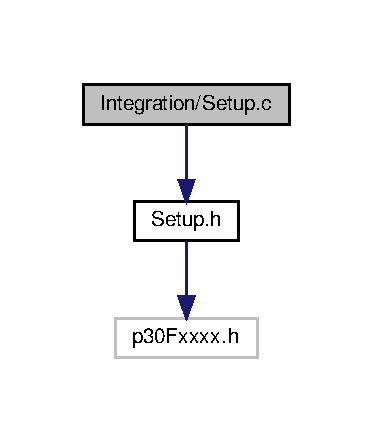
\includegraphics[width=179pt]{Setup_8c__incl}
\end{center}
\end{figure}
\subsection*{Functions}
\begin{DoxyCompactItemize}
\item 
\mbox{\Hypertarget{Setup_8c_ae73673b9808f19c5a743db0114edc0f5}\label{Setup_8c_ae73673b9808f19c5a743db0114edc0f5}} 
void \hyperlink{Setup_8c_ae73673b9808f19c5a743db0114edc0f5}{I\+O\+Setup} (void)
\begin{DoxyCompactList}\small\item\em IO Setup Function. \end{DoxyCompactList}\item 
\mbox{\Hypertarget{Setup_8c_ac9fec5d9a8b5a38b001b7eee4a68a502}\label{Setup_8c_ac9fec5d9a8b5a38b001b7eee4a68a502}} 
void \hyperlink{Setup_8c_ac9fec5d9a8b5a38b001b7eee4a68a502}{P\+W\+M\+Setup} (void)
\begin{DoxyCompactList}\small\item\em P\+WM Setup Function. \end{DoxyCompactList}\item 
\mbox{\Hypertarget{Setup_8c_a9d556c9c42a88652deb3e03bbcac6208}\label{Setup_8c_a9d556c9c42a88652deb3e03bbcac6208}} 
void \hyperlink{Setup_8c_a9d556c9c42a88652deb3e03bbcac6208}{U\+A\+R\+T\+Setup} (void)
\begin{DoxyCompactList}\small\item\em U\+A\+RT Setup Function. \end{DoxyCompactList}\item 
void \hyperlink{Setup_8c_a59a0dc4fe0533ecf97d294150e0c5d8b}{A\+D\+C\+\_\+\+Setup} (void)
\begin{DoxyCompactList}\small\item\em A\+DC Setup Function. \end{DoxyCompactList}\item 
\mbox{\Hypertarget{Setup_8c_ae8c79f2bc8cdc2156c04789b1dc078a1}\label{Setup_8c_ae8c79f2bc8cdc2156c04789b1dc078a1}} 
void {\bfseries timer1\+Setup} (void)
\end{DoxyCompactItemize}


\subsection{Detailed Description}
Functions and Definitions for peripheral systems. 

\begin{DoxyAuthor}{Author}
Christian Woof @ U\+WE Robotics 
\end{DoxyAuthor}


\subsection{Function Documentation}
\mbox{\Hypertarget{Setup_8c_a59a0dc4fe0533ecf97d294150e0c5d8b}\label{Setup_8c_a59a0dc4fe0533ecf97d294150e0c5d8b}} 
\index{Setup.\+c@{Setup.\+c}!A\+D\+C\+\_\+\+Setup@{A\+D\+C\+\_\+\+Setup}}
\index{A\+D\+C\+\_\+\+Setup@{A\+D\+C\+\_\+\+Setup}!Setup.\+c@{Setup.\+c}}
\subsubsection{\texorpdfstring{A\+D\+C\+\_\+\+Setup()}{ADC\_Setup()}}
{\footnotesize\ttfamily void A\+D\+C\+\_\+\+Setup (\begin{DoxyParamCaption}\item[{void}]{ }\end{DoxyParamCaption})}



A\+DC Setup Function. 

Timer 1 Setup Function. 
\hypertarget{main_8c}{}\section{main.\+c File Reference}
\label{main_8c}\index{main.\+c@{main.\+c}}


this is the main file that controls the robot.  


{\ttfamily \#include \char`\"{}Algorithm/\+Mapping\+Functions.\+h\char`\"{}}\newline
{\ttfamily \#include \char`\"{}Algorithm/\+Map\+Maze.\+h\char`\"{}}\newline
{\ttfamily \#include \char`\"{}Algorithm/\+Dijekstra.\+h\char`\"{}}\newline
{\ttfamily \#include $<$stdlib.\+h$>$}\newline
{\ttfamily \#include $<$stdio.\+h$>$}\newline
Include dependency graph for main.\+c\+:
\nopagebreak
\begin{figure}[H]
\begin{center}
\leavevmode
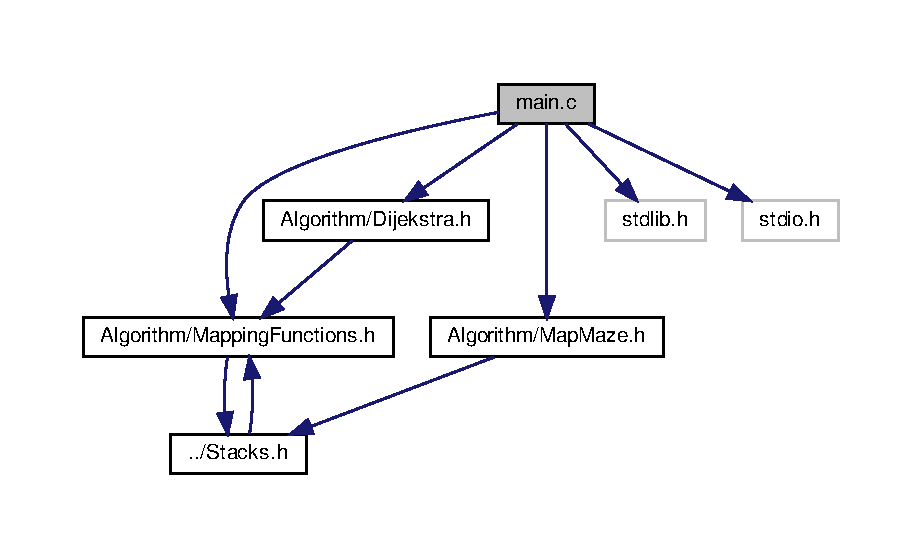
\includegraphics[width=350pt]{main_8c__incl}
\end{center}
\end{figure}
\subsection*{Functions}
\begin{DoxyCompactItemize}
\item 
\mbox{\Hypertarget{main_8c_ad515c06f1e515ece323faa50221347f2}\label{main_8c_ad515c06f1e515ece323faa50221347f2}} 
{\bfseries \+\_\+\+F\+W\+DT} (W\+D\+T\+\_\+\+O\+FF)
\item 
int \hyperlink{main_8c_a840291bc02cba5474a4cb46a9b9566fe}{main} (void)
\begin{DoxyCompactList}\small\item\em main. \end{DoxyCompactList}\end{DoxyCompactItemize}


\subsection{Detailed Description}
this is the main file that controls the robot. 

Contains the mission planner and runs all initialisation of maze. offloads most functionality to external functions.

\begin{DoxyAuthor}{Author}
Nick Appleton @ U\+WE Robotics
\end{DoxyAuthor}
\begin{DoxyDate}{Date}
21/2/19 
\end{DoxyDate}


\subsection{Function Documentation}
\mbox{\Hypertarget{main_8c_a840291bc02cba5474a4cb46a9b9566fe}\label{main_8c_a840291bc02cba5474a4cb46a9b9566fe}} 
\index{main.\+c@{main.\+c}!main@{main}}
\index{main@{main}!main.\+c@{main.\+c}}
\subsubsection{\texorpdfstring{main()}{main()}}
{\footnotesize\ttfamily int main (\begin{DoxyParamCaption}\item[{void}]{ }\end{DoxyParamCaption})}



main. 

\begin{DoxyReturn}{Returns}

\end{DoxyReturn}

\hypertarget{Stacks_8h}{}\section{Stacks.\+h File Reference}
\label{Stacks_8h}\index{Stacks.\+h@{Stacks.\+h}}


Defines everything needed to implement stacks.  


{\ttfamily \#include \char`\"{}Algorithm/\+Mapping\+Functions.\+h\char`\"{}}\newline
Include dependency graph for Stacks.\+h\+:
\nopagebreak
\begin{figure}[H]
\begin{center}
\leavevmode
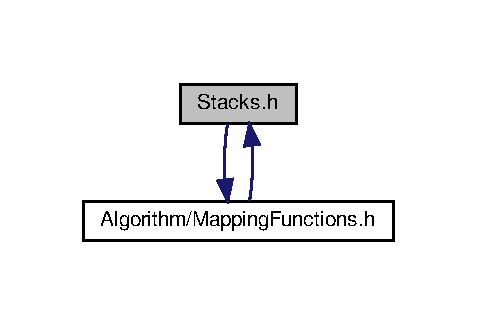
\includegraphics[width=229pt]{Stacks_8h__incl}
\end{center}
\end{figure}
This graph shows which files directly or indirectly include this file\+:
\nopagebreak
\begin{figure}[H]
\begin{center}
\leavevmode
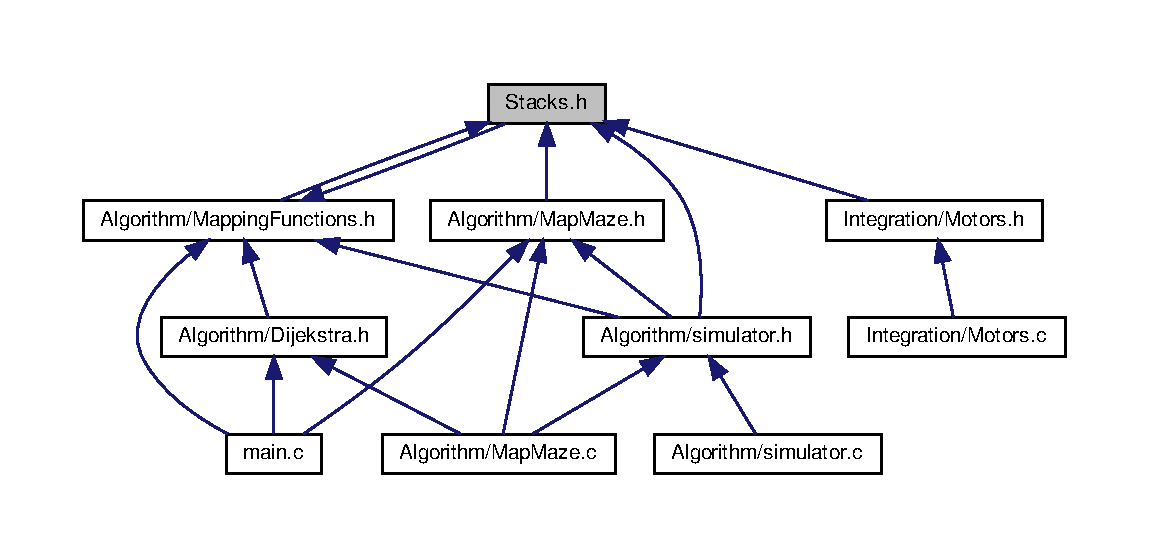
\includegraphics[width=350pt]{Stacks_8h__dep__incl}
\end{center}
\end{figure}
\subsection*{Classes}
\begin{DoxyCompactItemize}
\item 
struct \hyperlink{structStack}{Stack}
\begin{DoxyCompactList}\small\item\em array of data that is the \hyperlink{structStack}{Stack}. \end{DoxyCompactList}\end{DoxyCompactItemize}
\subsection*{Typedefs}
\begin{DoxyCompactItemize}
\item 
typedef struct \hyperlink{structStack}{Stack} \hyperlink{Stacks_8h_a16531b789dabfb1be2e263aa3c274df5}{Stack}
\begin{DoxyCompactList}\small\item\em array of data that is the \hyperlink{structStack}{Stack}. \end{DoxyCompactList}\end{DoxyCompactItemize}


\subsection{Detailed Description}
Defines everything needed to implement stacks. 

Includes the stack datatype, as well as the stackitem structure used to creat stacks. Stacks can have data pushed to them and popped from them. Uses Linked lists to do this.

\begin{DoxyAuthor}{Author}
Nick Appleton @ U\+WE Robotics
\end{DoxyAuthor}
\begin{DoxyDate}{Date}
23/2/19 
\end{DoxyDate}


\subsection{Typedef Documentation}
\mbox{\Hypertarget{Stacks_8h_a16531b789dabfb1be2e263aa3c274df5}\label{Stacks_8h_a16531b789dabfb1be2e263aa3c274df5}} 
\index{Stacks.\+h@{Stacks.\+h}!Stack@{Stack}}
\index{Stack@{Stack}!Stacks.\+h@{Stacks.\+h}}
\subsubsection{\texorpdfstring{Stack}{Stack}}
{\footnotesize\ttfamily typedef struct \hyperlink{structStack}{Stack}  \hyperlink{structStack}{Stack}}



array of data that is the \hyperlink{structStack}{Stack}. 

The size of the stack equal to number of cells in the maze. 
%--- End generated contents ---

% Index
\backmatter
\newpage
\phantomsection
\clearemptydoublepage
\addcontentsline{toc}{chapter}{Index}
\printindex

\end{document}
